%% LeJEPA Presentation Slides
%% Template: WASA-style (Metropolis) × LeJEPA color scheme
%% Compile: xelatex lejepa_slides.tex (twice)

\documentclass[aspectratio=169,9pt]{beamer}

\usetheme{metropolis}
\usepackage{fontspec}
\setmainfont{Latin Modern Sans}
\setsansfont{Latin Modern Sans}
\usepackage{amsmath,amssymb,bm}
\usepackage{booktabs}
\usepackage{tikz}
\usepackage{tikz-3dplot}
\usetikzlibrary{
  arrows.meta, positioning, shapes.geometric, fit, backgrounds,
  calc, decorations.pathreplacing, decorations.markings, patterns, 3d
}
\usepackage{pgfplots}
\pgfplotsset{compat=1.18}
\usepackage{xcolor}
\usepackage{colortbl}
\usepackage{graphicx}
\graphicspath{{figures/}}
\usepackage{mathtools}
\usepackage{mdframed}
\usepackage{array}
\usepackage{pifont}
\usepackage{listings}
\usepackage[numbers,compress]{natbib}
\renewcommand{\bibfont}{\tiny}
\newcommand{\cmark}{\ding{51}}
\newcommand{\xmark}{\ding{55}}

%% ─── Color Palette: WASA-style + LeJEPA Navy/Gold ───────────────────────────
\definecolor{mprimary}{HTML}{2C3E6B}   % Navy (LeJEPA primary)
\definecolor{maccent}{HTML}{C8A951}    % Gold
\definecolor{mgood}{HTML}{5B8C6B}      % Sage green
\definecolor{mbad}{HTML}{B85450}       % Terracotta
\definecolor{mgray}{HTML}{9E9E9E}      % Mid gray
\definecolor{mdark}{HTML}{212121}      % Near-black (header)
\definecolor{mlight}{HTML}{EEF0F5}     % Light blue-gray
\definecolor{mlightgold}{HTML}{F5F0E0} % Light gold
\definecolor{mlightsage}{HTML}{E5EDE8} % Light sage
\definecolor{mlightred}{HTML}{F2E6E5}  % Light terracotta

\setbeamercolor{frametitle}{bg=mdark, fg=white}
\setbeamercolor{progress bar}{fg=mprimary}
\setbeamercolor{structure}{fg=mprimary}
\setbeamercolor{title separator}{fg=maccent}

%% ─── mdframed Box Styles ─────────────────────────────────────────────────────
\newmdenv[
  topline=false, bottomline=false, rightline=false,
  linewidth=3pt, linecolor=mprimary!60,
  innerleftmargin=10pt, innerrightmargin=6pt,
  innertopmargin=5pt, innerbottommargin=5pt,
  backgroundcolor=mlight
]{primarybox}

\newmdenv[
  topline=false, bottomline=false, rightline=false,
  linewidth=3pt, linecolor=mgood!70,
  innerleftmargin=10pt, innerrightmargin=6pt,
  innertopmargin=5pt, innerbottommargin=5pt,
  backgroundcolor=mlightsage
]{goodbox}

\newmdenv[
  topline=false, bottomline=false, rightline=false,
  linewidth=3pt, linecolor=mbad!70,
  innerleftmargin=10pt, innerrightmargin=6pt,
  innertopmargin=5pt, innerbottommargin=5pt,
  backgroundcolor=mlightred
]{badbox}

\newmdenv[
  topline=false, bottomline=false, rightline=false,
  linewidth=3pt, linecolor=maccent!80,
  innerleftmargin=10pt, innerrightmargin=6pt,
  innertopmargin=5pt, innerbottommargin=5pt,
  backgroundcolor=mlightgold
]{accentbox}


\newmdenv[
  linewidth=1.6pt, linecolor=mgood!85!mprimary,
  roundcorner=3pt,
  innerleftmargin=10pt, innerrightmargin=8pt,
  innertopmargin=6pt, innerbottommargin=6pt,
  backgroundcolor=mlightsage
]{insightbox}

\newcommand{\kw}[1]{\textbf{\color{mprimary}#1}}

%% ─── Takeaway Banner ─────────────────────────────────────────────────────────
\newcommand{\takeaway}[1]{%
  \vfill
  \begin{mdframed}[
    linecolor=maccent, linewidth=1.5pt,
    backgroundcolor=mlightgold,
    innertopmargin=5pt, innerbottommargin=5pt,
    innerleftmargin=10pt, innerrightmargin=10pt,
    roundcorner=3pt, skipabove=4pt, skipbelow=0pt
  ]
  \centering\small\bfseries\color{mprimary} #1
  \end{mdframed}%
}

%% ─── TikZ styles ─────────────────────────────────────────────────────────────
\tikzset{
  pbox/.style={draw=mprimary!50, fill=mlight, rounded corners=3pt,
               minimum height=0.65cm, font=\small, inner sep=5pt},
  gbox/.style={draw=mgood!60, fill=mlightsage, rounded corners=3pt,
               minimum height=0.65cm, font=\small, inner sep=5pt},
  rbox/.style={draw=mbad!60, fill=mlightred, rounded corners=3pt,
               minimum height=0.65cm, font=\small, inner sep=5pt},
  abox/.style={draw=maccent!70, fill=mlightgold, rounded corners=3pt,
               minimum height=0.65cm, font=\small, inner sep=5pt},
  darkbox/.style={draw=mprimary, fill=mprimary!85, text=white, rounded corners=3pt,
                  minimum height=0.7cm, font=\small\bfseries, inner sep=6pt},
  arr/.style={->, thick, mprimary},
  darr/.style={->, dashed, thin, mgray},
}

%% ─── Title ───────────────────────────────────────────────────────────────────
\title{\textbf{LeJEPA}\\
       \large Provable \& Scalable Self-Supervised Learning}
\subtitle{Without the Heuristics \quad\textcolor{mgray}{\small Balestriero \& LeCun, arXiv:2511.08544}}
\author{}
\date{}

% ═══════════════════════════════════════════════════════════════════════════════
\begin{document}
% ═══════════════════════════════════════════════════════════════════════════════

% ─── Title Slide (custom) ─────────────────────────────────────────────────────
\begin{frame}[plain]
\vspace{0.4cm}
\begin{columns}[c]
\column{0.48\textwidth}
  \begin{center}
    {\Huge\bfseries\color{mprimary} LeJEPA}\\[6pt]
    {\large\itshape\color{mprimary!80} Provable \& Scalable SSL}\\[4pt]
    {\normalsize\itshape Without the Heuristics}\\[14pt]
    {\small\color{mgray} Randall Balestriero \& Yann LeCun (2025)}\\[3pt]
    {\small\color{mgray} arXiv:~2511.08544}\\[12pt]
    {\small\bfseries\color{mprimary} Presenter: Continuer team}
  \end{center}

\column{0.50\textwidth}
\begin{center}
\begin{tikzpicture}[every node/.style={font=\small}, scale=0.95]

  %% Input — fan-stacked photos (back to front)
  \begin{scope}[yshift=0.12cm]
    % Back photo: navy, tilted -14°
    \begin{scope}[rotate around={-14:(-0.12,0)}]
      \fill[mprimary!11, rounded corners=3pt] (-0.59,-0.62) rectangle (0.35,0.62);
      \fill[mprimary!23]                      (-0.59, 0.08) rectangle (0.35,0.62);
      \fill[mprimary!38, opacity=0.72]        (-0.12,-0.16) ellipse (0.17 and 0.21);
      \draw[mprimary!32, line width=0.6pt, rounded corners=3pt] (-0.59,-0.62) rectangle (0.35,0.62);
    \end{scope}

    % Middle photo: sage, tilted +7°
    \begin{scope}[rotate around={7:(0.10,-0.05)}]
      \fill[mgood!10, rounded corners=3pt] (-0.37,-0.67) rectangle (0.57,0.57);
      \fill[mgood!20]                      (-0.37, 0.05) rectangle (0.57,0.57);
      \fill[mgood!38, opacity=0.72]        (0.10,-0.18) ellipse (0.17 and 0.21);
      \draw[mgood!33, line width=0.6pt, rounded corners=3pt] (-0.37,-0.67) rectangle (0.57,0.57);
    \end{scope}

    % Front photo: warm gold, straight
    \fill[maccent!11, rounded corners=3pt] (-0.19,-0.72) rectangle (0.75,0.48);
    \fill[maccent!23]                      (-0.19,-0.04) rectangle (0.75,0.48);
    \fill[maccent!42, opacity=0.72]        (0.28,-0.24) ellipse (0.17 and 0.21);
    \draw[maccent!38, line width=0.6pt, rounded corners=3pt] (-0.19,-0.72) rectangle (0.75,0.48);

    % Invisible anchor for label
    \node[inner sep=0, minimum width=2.0cm, minimum height=1.5cm] (img) at (0.08,-0.10) {};
    \node[font=\tiny, mgray, below=6pt of img] {Dữ liệu};
  \end{scope}

  %% Encoder box
  \node[darkbox, minimum width=1.1cm, minimum height=0.75cm] (enc) at (2.2,0) {$f_\theta$};
  \node[font=\tiny, mgray, below=3pt of enc] {Bộ mã hóa};

  %% Arrow: right edge of front photo → enc
  \draw[->, thick, mprimary] (0.77, 0) -- (enc.west);

  %% Embedding dots
  \fill[mgood!80] (4.0,  0.0) circle (4.5pt);
  \fill[mgood!80] (4.45, 0.7) circle (3.8pt);
  \fill[mgood!80] (4.5, -0.6) circle (4.2pt);
  \fill[mgood!80] (5.05, 0.3) circle (3.4pt);
  \fill[mgood!80] (4.95,-1.0) circle (3.8pt);

  %% Dashed Gaussian circle
  \draw[dashed, mgood!60, line width=1.1pt] (4.55, -0.18) circle (1.38cm);
  \node[font=\scriptsize, mgood] at (5.85, 1.05) {$\mathcal{N}(0,I)$};

  %% Arrows enc -> embeddings
  \foreach \x/\y in {4.0/0.0, 4.45/0.7, 4.5/-0.6, 5.05/0.3, 4.95/-1.0}{
    \draw[->, thick, mgood!70] (enc.east) -- (\x,\y);
  }

\end{tikzpicture}
\end{center}
\end{columns}
\end{frame}

\begin{frame}{Nội Dung Trình Bày}
\vspace{0.6cm}
\begin{center}
\begin{tikzpicture}[x=2.35cm, y=1cm]
  \tikzstyle{stepbox} = [draw=mprimary!40, fill=white, rounded corners=6pt, text width=1.85cm, align=center, inner sep=4pt, minimum height=1.25cm, line width=1.1pt]
  \tikzstyle{stepnum} = [circle, fill=mprimary, text=white, font=\normalsize\bfseries, inner sep=0pt, minimum size=0.65cm]

  %% Một đường thẳng duy nhất nối 5 bước
  \draw[line width=1.6pt, mprimary!20] (0, 1.5) -- (4, 1.5);

  %% Step 1
  \node[stepbox, draw=mprimary] (b1) at (0, -0.1) {\small\textbf{\color{mprimary}WHAT}\\[2pt]\scriptsize Học biểu diễn là gì?};
  \node[stepnum, fill=mprimary] (n1) at (0, 1.5) {1};
  \draw[thick, mprimary] (n1) -- (b1);
  %% Step 2
  \node[stepbox, draw=mbad] (b2) at (1, -0.1) {\small\textbf{\color{mbad}WHY}\\[2pt]\scriptsize Tại sao JEPA thất bại?};
  \node[stepnum, fill=mbad] (n2) at (1, 1.5) {2};
  \draw[thick, mbad] (n2) -- (b2);
  %% Step 3
  \node[stepbox, draw=mgood] (b3) at (2, -0.1) {\small\textbf{\color{mgood}HOW}\\[2pt]\scriptsize Giải quyết từ gốc rễ};
  \node[stepnum, fill=mgood] (n3) at (2, 1.5) {3};
  \draw[thick, mgood] (n3) -- (b3);
  %% Step 4
  \node[stepbox, draw=maccent] (b4) at (3, -0.1) {\small\textbf{\color{maccent}KẾT QUẢ}\\[2pt]\scriptsize Đánh giá thực nghiệm};
  \node[stepnum, fill=maccent] (n4) at (3, 1.5) {4};
  \draw[thick, maccent] (n4) -- (b4);
  %% Step 5
  \node[stepbox, draw=mprimary!85!mgood] (b5) at (4, -0.1) {\small\textbf{\color{mprimary!85!mgood}MỞ RỘNG}\\[2pt]\scriptsize Benchmark Climb};
  \node[stepnum, fill=mprimary!85!mgood] (n5) at (4, 1.5) {5};
  \draw[thick, mprimary!85!mgood] (n5) -- (b5);

\end{tikzpicture}
\end{center}

\vspace{0.5cm}
\begin{accentbox}
\centering\small
\textit{“LeJEPA: Tối giản hóa self-supervised learning bằng nền tảng lý thuyết vững chắc.”}
\end{accentbox}
\end{frame}

% ─── Slide: Short Glossary ───────────────────────────────────────────────────
\begin{frame}{Thuật Ngữ Trọng Tâm}
  \vspace{0.3em}
  Các khái niệm cốt lõi thường xuyên xuất hiện trong bài trình bày:
  
  \vspace{0.6em}
  \begin{enumerate}\small\setlength\itemsep{1em}
    \item \textbf{\color{mprimary}Anisotropic / Isotropic:} Bất đẳng hướng (các hướng không đều) / Đẳng hướng (phân bố đều mọi hướng).
    \item \textbf{\color{mprimary}SSL:} Self-Supervised Learning (Học máy tự giám sát).
    \item \textbf{\color{mprimary}Random projection:} Phép chiếu ngẫu nhiên (chuyển không gian dữ liệu nhiều chiều xuống ít chiều hơn).
    \item \textbf{\color{mprimary}Decision boundary:} Ranh giới quyết định (đường/mặt phân tách các nhóm dữ liệu trong mô hình).
    \item \textbf{\color{mprimary}Exploding gradients:} Bùng nổ đạo hàm (đạo hàm tăng quá lớn khiến mô hình không thể huấn luyện).
  \end{enumerate}
\end{frame}


% ─── SECTION DIVIDER ──────────────────────────────────────────────────────────
\section{WHAT — Học biểu diễn là gì?}

% ─── Slide 1: Foundation model goal ──────────────────────────────────────────
\begin{frame}{Mục Tiêu: Encoder Ánh Xạ Thế Giới Vào Không Gian Có Ý Nghĩa}

\begin{columns}[T]
\column{0.50\textwidth}

Học $f_\theta : \mathbb{R}^D \to \mathbb{R}^K$ sao cho embedding \textbf{có ích cho mọi downstream task} — không cần nhãn trong lúc huấn luyện.

\vspace{0.7em}
\begin{tikzpicture}[scale=0.88, every node/.style={font=\small}]
  %% Input
  \node[pbox, minimum width=1.0cm] (x) at (0,0) {$\mathbf{x}$};
  \node[font=\tiny, mgray, below=2pt of x] {ảnh / video / text};

  %% Encoder
  \node[darkbox, minimum width=1.3cm, minimum height=1.0cm] (enc) at (2.3,0) {$f_\theta$};

  %% Latent space — ink-blot shape
  \begin{scope}[xshift=4.2cm, yshift=0cm]
    \node[font=\tiny, mgray] at (0.8, 1.15) {$\mathbb{R}^K$};
    % Blob
    \draw[mprimary!25, fill=mprimary!7, thick, line width=1pt]
      plot[smooth cycle, tension=0.75] coordinates {
        (0.1,0.3) (0.2,0.9) (0.6,1.0) (1.1,0.85)
        (1.6,0.65) (1.7,0.1) (1.2,-0.35) (0.6,-0.4) (0.0,-0.1)
      };
    % Clusters of dots
    \foreach \x/\y/\c in {
      0.35/0.55/mgood, 0.55/0.75/mgood, 0.4/0.85/mgood,
      1.0/0.65/mprimary, 1.2/0.5/mprimary, 1.1/0.3/mprimary,
      0.75/0.0/maccent, 0.6/-0.2/maccent}{
      \fill[\c, opacity=0.85] (\x,\y) circle (2.2pt);
    }
    % Cluster labels
    \node[font=\tiny, mgood]   at (0.35,0.35) {cat};
    \node[font=\tiny, mprimary] at (1.3,0.7)  {dog};
    \node[font=\tiny, maccent]  at (0.55,-0.35){sky};
  \end{scope}

  \draw[arr] (x) -- (enc);
  \draw[arr] (enc) -- (4.0, 0);
\end{tikzpicture}

\column{0.47\textwidth}
\vspace{0.4em}

Một $f_\theta$ tốt phục vụ được nhiều task:

\vspace{0.4em}
\begin{tikzpicture}[every node/.style={font=\footnotesize}, scale=0.88]
  \node[pbox, minimum width=0.7cm] (z) at (0,0) {$\mathbf{z}$};
  \foreach \ang/\lbl/\col in {
    70/Phân loại/mgood,
    10/Segmentation/mprimary,
    -45/Few-shot/maccent,
    -100/Retrieval/mgray}{
    \node[\col!90, align=left] (t) at (\ang:2.4cm) {\lbl};
    \draw[->, thin, \col!60] (z) -- (t);
  }
\end{tikzpicture}

\end{columns}

\vspace{0.3em}
\begin{primarybox}
\footnotesize \textbf{Foundation model:} một hệ thống giải được nhiều downstream task sau khi huấn luyện một lần, không thay đổi tham số $\theta$.
\end{primarybox}

\end{frame}


% ─── Slide 2: JEPA mechanism ─────────────────────────────────────────────────
\begin{frame}{JEPA: Dự Đoán Trạng Thái Trừu Tượng — Không Phải Pixel}

\begin{columns}[T]
\column{0.56\textwidth}

\vspace{0.3em}
\begin{tikzpicture}[every node/.style={font=\tiny}, scale=0.82, transform shape]
  % Ảnh gốc
  \node[pbox, minimum width=0.9cm, minimum height=0.55cm] (src) at (0.0, 0.0) {$x$};
  \node[font=\tiny, below=3pt of src] {Ảnh gốc};
  % Views
  \node[pbox, minimum width=0.9cm, minimum height=0.55cm] (v1) at (1.4,  0.7) {view 1};
  \node[pbox, minimum width=0.9cm, minimum height=0.55cm] (v2) at (1.4, -0.7) {view 2};
  \draw[darr] (src.north east) -- (v1.west);
  \draw[darr] (src.south east) -- (v2.west);
  % Encoders
  \node[darkbox, minimum width=0.9cm, minimum height=0.55cm] (e1) at (2.8,  0.7) {$f_\theta$};
  \node[darkbox, minimum width=0.9cm, minimum height=0.55cm] (e2) at (2.8, -0.7) {$f_\theta$};
  \draw[arr] (v1) -- (e1);
  \draw[arr] (v2) -- (e2);
  % Latents
  \node[abox, minimum width=0.7cm, minimum height=0.55cm] (z1) at (4.0,  0.7) {$z_1$};
  \node[abox, minimum width=0.7cm, minimum height=0.55cm] (z2) at (4.0, -0.7) {$z_2$};
  \draw[arr] (e1) -- (z1);
  \draw[arr] (e2) -- (z2);
  % Predictor + ẑ_1
  \node[darkbox, minimum width=1.1cm, minimum height=0.55cm] (pred) at (5.4, -0.7) {Dự báo};
  \node[abox,  minimum width=0.7cm, minimum height=0.55cm] (zh)   at (6.8, -0.7) {$\hat{z}_1$};
  \draw[arr] (z2)   -- (pred);
  \draw[arr] (pred) -- (zh);
  % Loss
  \node[gbox, draw=mgood!80, text=mprimary, font=\small\bfseries,
        minimum width=1.1cm, minimum height=0.65cm] (loss) at (8.2, -0.7) {Loss};
  \draw[arr] (zh) -- (loss);
  % z1 → loss: đi ngang hàng trên rồi thả xuống
  \draw[arr] (z1.east) -- (8.2, 0.7) -- (loss.north);
  % Shared encoder background
  \begin{pgfonlayer}{background}
    \node[draw=mgray, dashed, fill=mgray!5, rounded corners=4pt,
          fit=(e1)(e2), inner sep=5pt] (encbox) {};
  \end{pgfonlayer}
  \node[font=\tiny, color=mgray, above=3pt of encbox] {chia sẻ trọng số};
\end{tikzpicture}

\column{0.41\textwidth}
\vspace{0.5em}

\textbf{View} có thể là: crop, mask, blur, frame liền kề, modal khác…

\vspace{0.6em}
\begin{goodbox}
\footnotesize \textbf{JEPA} $\neq$ reconstruction: không khôi phục pixel mà học ``thế giới thay đổi thế nào'' ở mức trừu tượng.
\end{goodbox}

\vspace{0.6em}
Tuy nhiên, bài toán dự đoán có một \textbf{nghiệm tầm thường nguy hiểm}…

\end{columns}

\takeaway{JEPA: học trạng thái latent — không học pixel}

\end{frame}


% ─── SECTION DIVIDER ──────────────────────────────────────────────────────────
\section{WHY — Tại sao JEPA thất bại?}


% ─── Slide 3: Collapse explained ─────────────────────────────────────────────
\begin{frame}{Collapse — Khi Encoder Học Cách "Gian Lận"}

Việc cực tiểu hóa loss prediction $\|z_1 - \hat z_1\|^2$ có nghiệm hiển nhiên: \textbf{Collapse}. Mọi input đều bị ánh xạ về một cấu trúc vô dụng, loss giảm về 0 nhưng encoder không học được gì.

\vspace{0.4cm}
\begin{center}
\begin{tikzpicture}[every node/.style={font=\small}, scale=0.9]

  %% Subfig 1: Complete Collapse
  \node[mbad, font=\small\bfseries] at (0, 2.5) {Complete Collapse};
  % Input dots converging to one point
  \foreach \x/\y in {-1.5/1.2, -0.8/1.6, 0/1.4, 0.8/1.6, 1.5/1.2, -0.4/0.9, 0.4/0.9}{
    \fill[mbad!50] (\x,\y) circle (2.5pt);
    \draw[->, very thin, mbad!40] (\x,\y-0.15) -- (0, 0.15);
  }
  % Collapsed point
  \fill[mbad] (0,0) circle (6pt);
  \node[mbad, font=\scriptsize\bfseries, below=4pt] at (0,0) {$f_\theta(\mathbf{x}) = c \;\; \forall \mathbf{x}$};

  %% Separator
  \draw[dashed, mgray!40] (3.5, -0.5) -- (3.5, 2.8);

  %% Subfig 2: Dimensional Collapse
  \node[maccent, font=\small\bfseries] at (7, 2.5) {Dimensional Collapse};
  % A flat 1D line in 2D space
  \draw[thick, maccent!40] (4.5, 0.5) -- (9.5, 0.5);
  % Dots mapped onto the line only
  \foreach \x in {4.8, 5.5, 6.1, 7.0, 7.8, 8.5, 9.2}{
    \fill[maccent] (\x,0.5) circle (3.5pt);
  }
  \node[maccent, font=\scriptsize\bfseries, below=4pt] at (7,0.5) {Sống trên không gian con chiều thấp};

\end{tikzpicture}
\end{center}

\vspace{0.2cm}
\begin{columns}[T]
\column{0.48\textwidth}
\begin{badbox}
\footnotesize \textbf{Complete collapse:}\\ Mất toàn bộ thông tin về input.
\end{badbox}

\column{0.48\textwidth}
\begin{accentbox}
\footnotesize \textbf{Dimensional collapse:}\\ Representation kém đa dạng, downstream task hỏng.
\end{accentbox}
\end{columns}

\vspace{0.5cm}
\begin{center}
\footnotesize \textbf{Vấn đề:} Không có lý thuyết nào chỉ ra \emph{chính xác} phải làm gì để tránh collapse \textbf{mà vẫn tối ưu} cho downstream task.
\end{center}

\end{frame}


% ─── Slide 4: Literature timeline ────────────────────────────────────────────
\begin{frame}{Literature: Mỗi Phương Pháp Vá Một Lỗ Hổng Mới}

\vfill
\begin{center}
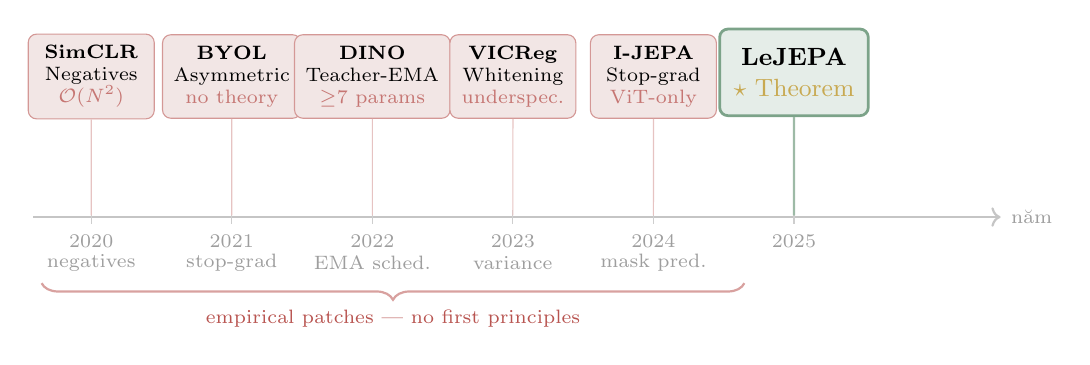
\begin{tikzpicture}[scale=1.05, every node/.style={font=\small}]
  %% Timeline axis
  \draw[->, thick, mgray!60] (-0.2,0) -- (11.5,0)
    node[right, mgray, font=\scriptsize]{năm};
  \foreach \x/\yr in {0.5/2020, 2.2/2021, 3.9/2022, 5.6/2023, 7.3/2024, 9.0/2025}{
    \draw[mgray!50] (\x,0.08) -- (\x,-0.08);
    \node[mgray, font=\scriptsize, below=3pt] at (\x,0) {\yr};
  }

  %% Heuristic method boxes — slightly taller for readability
  \node[rbox, minimum width=1.6cm, minimum height=1.0cm, align=center, font=\scriptsize, inner sep=4pt]
    (mA) at (0.5,1.7) {\textbf{SimCLR}\\Negatives\\\textcolor{mbad!80}{$\mathcal{O}(N^2)$}};
  \draw[mbad!35,thin] (mA.south)--(0.5,0.02);

  \node[rbox, minimum width=1.6cm, minimum height=1.0cm, align=center, font=\scriptsize, inner sep=4pt]
    (mB) at (2.2,1.7) {\textbf{BYOL}\\Asymmetric\\\textcolor{mbad!80}{no theory}};
  \draw[mbad!35,thin] (mB.south)--(2.2,0.02);

  \node[rbox, minimum width=1.6cm, minimum height=1.0cm, align=center, font=\scriptsize, inner sep=4pt]
    (mC) at (3.9,1.7) {\textbf{DINO}\\Teacher-EMA\\\textcolor{mbad!80}{$\geq$7 params}};
  \draw[mbad!35,thin] (mC.south)--(3.9,0.02);

  \node[rbox, minimum width=1.6cm, minimum height=1.0cm, align=center, font=\scriptsize, inner sep=4pt]
    (mD) at (5.6,1.7) {\textbf{VICReg}\\Whitening\\\textcolor{mbad!80}{underspec.}};
  \draw[mbad!35,thin] (mD.south)--(5.6,0.02);

  \node[rbox, minimum width=1.6cm, minimum height=1.0cm, align=center, font=\scriptsize, inner sep=4pt]
    (mE) at (7.3,1.7) {\textbf{I-JEPA}\\Stop-grad\\\textcolor{mbad!80}{ViT-only}};
  \draw[mbad!35,thin] (mE.south)--(7.3,0.02);

  %% LeJEPA — highlight, taller
  \node[gbox, minimum width=1.75cm, minimum height=1.1cm, align=center,
        draw=mgood!80, line width=1pt, font=\small, inner sep=5pt]
    (lj) at (9.0, 1.75)
    {\textbf{LeJEPA}\\\textcolor{maccent}{$\star$ Theorem}};
  \draw[mgood!60, thick] (lj.south) -- (9.0, 0.02);

  %% Patch labels below axis
  \foreach \x/\lbl in {
    0.5/negatives, 2.2/stop-grad, 3.9/EMA sched., 5.6/variance, 7.3/mask pred.}{
    \node[mgray, font=\scriptsize] at (\x, -0.55) {\lbl};
  }

  %% Brace
  \draw[decorate, decoration={brace, mirror, amplitude=6pt}, mbad!55, thick]
    (-0.1,-0.8) -- (8.4,-0.8)
    node[midway, below=6pt, font=\scriptsize, mbad]
      {empirical patches — no first principles};

\end{tikzpicture}
\end{center}
\vfill
\takeaway{Câu hỏi sai: \emph{``tránh collapse thế nào?''} $\;\longrightarrow\;$ Câu hỏi đúng: \emph{``phân phối nào là tối ưu?''}}

\end{frame}


% ─── SECTION DIVIDER ──────────────────────────────────────────────────────────
\section{HOW — Giải từ gốc rễ}


% ─── Slide 5: The right question ─────────────────────────────────────────────
\begin{frame}{Phân phối Nào Là Tối Ưu Cho Foundation Model?}

\begin{center}
Đánh giá downstream qua \textbf{linear probe} (ridge):\quad
$\hat\beta = \arg\min_\beta \|\mathbf{y} - \mathbf{Z}\beta\|^2 + \lambda\|\beta\|^2$
\end{center}

\vspace{0.6em}
\begin{center}
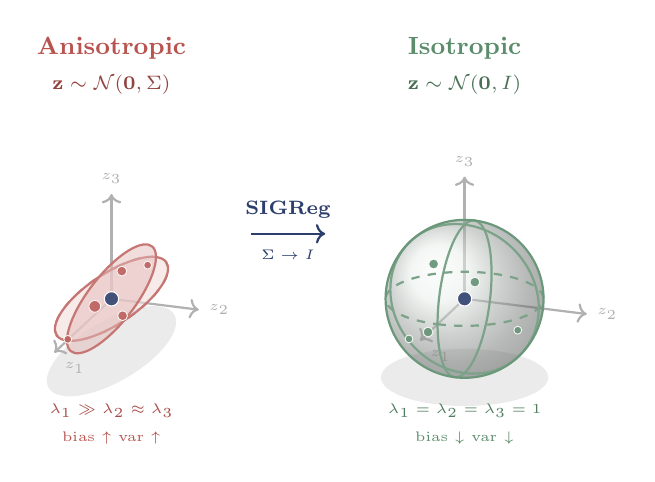
\begin{tikzpicture}[scale=1.18, every node/.style={font=\small}, line join=round]
  \tdplotsetmaincoords{70}{110}
  
  %% ── Anisotropic (left) ──
  \begin{scope}[xshift=1.0cm]
    \node[mbad, font=\small\bfseries] at (0, 2.5) {Anisotropic};
    \node[font=\scriptsize, mbad!80!black] at (0, 2.1) {$\mathbf{z} \sim \mathcal{N}(\mathbf{0}, \Sigma)$};
    
    \begin{scope}[yshift=-0.2cm]
      \begin{scope}[tdplot_main_coords]
        % Shadow
        \begin{scope}[canvas is xy plane at z=-0.6]
          \fill[mgray!30, opacity=0.7] (0,0) ellipse (1.5cm and 0.5cm);
        \end{scope}
        
        % 3D Axes
        \draw[->, thick, mgray!80] (0,0,0) -- (1.8,0,0) node[anchor=north west, font=\tiny]{$z_1$};
        \draw[->, thick, mgray!80] (0,0,0) -- (0,1.0,0) node[anchor=west, font=\tiny]{$z_2$};
        \draw[->, thick, mgray!80] (0,0,0) -- (0,0,1.2) node[anchor=south, font=\tiny]{$z_3$};
        
        % Ellipsoid (Anisotropic)
        \begin{scope}[canvas is xy plane at z=0]
          \draw[mbad!80, thick, dashed] (0,0) ellipse (1.4cm and 0.4cm);
          \fill[mbad!20, opacity=0.6] (0,0) ellipse (1.4cm and 0.4cm);
          \draw[mbad!80, thick] (0,0) ellipse (1.4cm and 0.4cm);
        \end{scope}
        
        \begin{scope}[canvas is xz plane at y=0]
          \fill[mbad!40, opacity=0.5] (0,0) ellipse (1.4cm and 0.4cm);
          \draw[mbad!80, thick] (0,0) ellipse (1.4cm and 0.4cm);
        \end{scope}
        
        % Scatter Points (clean flat look with white outline)
        \tikzset{scatterpt/.style={fill=mbad!90, draw=white, line width=0.3pt, opacity=0.95}}
        \path[scatterpt] (0.8,0.1,0.2) circle (1.8pt);
        \path[scatterpt] (-0.6,-0.1,0.1) circle (1.5pt);
        \path[scatterpt] (0.2,0.2,-0.1) circle (1.5pt);
        \path[scatterpt] (-1.0,0.05,0.05) circle (1.2pt);
        \path[scatterpt] (1.1,-0.1,-0.1) circle (1.2pt);
        \fill[mprimary!90, draw=white, line width=0.4pt] (0,0,0) circle (2.2pt); % Center
      \end{scope}
    \end{scope}
    
    \node[font=\tiny, mbad!90!black, align=center] at (0, -1.4) {$\lambda_1 \gg \lambda_2 \approx \lambda_3$};
    \node[font=\tiny, mbad, align=center] at (0, -1.7) {bias $\uparrow$\ var $\uparrow$};
  \end{scope}

  %% Arrow
  \draw[->, thick, mprimary] (2.5, 0.5) -- (3.3, 0.5)
    node[above=2pt, midway, font=\scriptsize\bfseries]{SIGReg}
    node[below=2pt, midway, font=\tiny]{$\Sigma \to I$};

  %% ── Isotropic (right) ──
  \begin{scope}[xshift=4.8cm]
    \node[mgood, font=\small\bfseries] at (0, 2.5) {Isotropic};
    \node[font=\scriptsize, mgood!80!black] at (0, 2.1) {$\mathbf{z} \sim \mathcal{N}(\mathbf{0}, I)$};
    
    \begin{scope}[yshift=-0.2cm]
      \begin{scope}[tdplot_main_coords]
        % Shadow
        \begin{scope}[canvas is xy plane at z=-0.9]
          \fill[mgray!30, opacity=0.7] (0,0) circle (0.9cm);
        \end{scope}
        
        % 3D Axes
        \draw[->, thick, mgray!80] (0,0,0) -- (1.4,0,0) node[anchor=north west, font=\tiny]{$z_1$};
        \draw[->, thick, mgray!80] (0,0,0) -- (0,1.4,0) node[anchor=west, font=\tiny]{$z_2$};
        \draw[->, thick, mgray!80] (0,0,0) -- (0,0,1.4) node[anchor=south, font=\tiny]{$z_3$};
        
        % Sphere (Isotropic)
        \shade[ball color=mgood!20, opacity=0.5] (0,0,0) circle (0.85cm);
        
        \begin{scope}[canvas is xy plane at z=0]
          \draw[mgood!80, thick, dashed] (0,0) circle (0.85cm); 
        \end{scope}
        \begin{scope}[canvas is xz plane at y=0]
          \draw[mgood!80, thick] (0,0) circle (0.85cm);
        \end{scope}
        \begin{scope}[canvas is yz plane at x=0]
          \draw[mgood!80, thick] (0,0) circle (0.85cm);
        \end{scope}
      \end{scope}
      
      % Draw outer circle outside tdplot_main_coords so it's a perfect circle in screen space!
      \draw[mgood!90, thick] (0,0) circle (0.85cm);
      
      \begin{scope}[tdplot_main_coords]
        % Scatter Points (clean flat look with white outline)
        \tikzset{scatterpt2/.style={fill=mgood!90, draw=white, line width=0.3pt, opacity=0.95}}
        \path[scatterpt2] (0.5,0.3,0.4) circle (1.5pt);
        \path[scatterpt2] (-0.4,-0.5,0.2) circle (1.5pt);
        \path[scatterpt2] (-0.3,0.5,-0.4) circle (1.2pt);
        \path[scatterpt2] (0.1,-0.6,-0.5) circle (1.2pt);
        \path[scatterpt2] (0.6,-0.2,-0.2) circle (1.5pt);
        \fill[mprimary!90, draw=white, line width=0.4pt] (0,0,0) circle (2.2pt); % Center
      \end{scope}
    \end{scope}
    
    \node[font=\tiny, mgood!90!black, align=center] at (0, -1.4) {$\lambda_1 = \lambda_2 = \lambda_3 = 1$};
    \node[font=\tiny, mgood, align=center] at (0, -1.7) {bias $\downarrow$\ var $\downarrow$};
  \end{scope}
\end{tikzpicture}
\end{center}

\vfill
\begin{accentbox}
\footnotesize \textbf{Giả thuyết:} Isotropic Gaussian $\mathcal{N}(\mathbf{0}, I)$ tối ưu trên \emph{cả} bias \emph{lẫn} variance, cho \emph{mọi} downstream task.
\end{accentbox}

\end{frame}


% ─── [MERGED, giữ dạng backup] Tóm tắt gộp Bổ đề 1+2 + Định lý 1 + Kết luận ───
% Slide sau đây gộp nội dung thành 1 slide nhẹ toán; giữ comment lại vì merge
% cuối cùng ưu tiên bản đầy đủ, chi tiết hơn (4 frame riêng: Bổ đề 1, Bổ đề 2,
% Định lý 1, Kết Luận Lý Thuyết) ngay bên dưới thay vì bản tóm gọn này.
\iffalse
\begin{frame}{Tóm Tắt: Vì Sao Isotropic Gaussian Là Tối Ưu}

\vspace{0.4em}
\begin{center}
\begin{tikzpicture}[
    lemma/.style={draw=mbad!55, fill=mlightred, rounded corners=4pt,
                  text width=4.0cm, align=left, inner sep=6pt, font=\footnotesize,
                  minimum height=1.5cm},
    thm/.style={draw=mgood!70, fill=mlightsage, rounded corners=4pt,
                text width=4.8cm, align=left, inner sep=7pt, font=\footnotesize,
                minimum height=1.9cm},
    concl/.style={draw=mprimary, fill=mprimary!8, rounded corners=5pt,
                  align=center, inner sep=8pt},
  ]
  % Hai bổ đề (trái, xếp dọc)
  \node[lemma] (l1) at (0, 1.35) {\textbf{Bổ đề 1 · Bias$\,\uparrow$}\\[2pt]
    Trị riêng nhỏ $\to$ ridge co mạnh hơn.};
  \node[lemma] (l2) at (0, -1.35) {\textbf{Bổ đề 2 · Variance$\,\uparrow$}\\[2pt]
    Trị riêng lệch $\to$ boundary dao động.};

  % Định lý (giữa)
  \node[thm] (thm) at (7.6, 0) {\textbf{Định lý 1 — Duy nhất}\\[2pt]
    Cố định $\mathrm{Tr}(\mathrm{Cov})=\kappa$: $\mathcal{N}(0,\kappa I/K)$ là cực tiểu
    \textbf{duy nhất} — probe, kNN, kernel.};

  % Gộp 2 bổ đề → mũi tên ⇒ định lý
  \draw[thick, mbad!50] (l1.east) -| (3.6, 0);
  \draw[thick, mbad!50] (l2.east) -| (3.6, 0);
  \fill[mbad!50] (3.6, 0) circle (1.6pt);
  \draw[-{Latex[length=2.8mm]}, very thick, mprimary] (3.6, 0) -- (thm.west);

  % Kết luận: công thức (dưới, mũi tên xuống)
  \node[concl] (f) at (7.6, -2.7)
    {\large\bfseries\color{mprimary}$f_\theta(\mathbf{x}) \sim \mathcal{N}(\mathbf{0}, I)$};
  \draw[-{Latex[length=2.8mm]}, very thick, mgood!80] (thm.south) -- (f.north);
  \node[font=\scriptsize\itshape, mgray, below=3pt of f, align=center]
    {Design principle duy nhất cần đạt — không cần heuristic.};
\end{tikzpicture}
\end{center}

\takeaway{Anisotropy $\Rightarrow$ bias $\uparrow$ \& variance $\uparrow$ cho mọi downstream task — Isotropic Gaussian tối ưu mọi probe}

\end{frame}
\fi % ─── hết bản tóm tắt gộp (backup) ────────────────────────────────────────


% ═══ Shared helpers cho vòng cung lý thuyết (Bổ đề 1 · Bổ đề 2 · Định lý 1) ═══
% Progress ribbon: 3 chặng, chặng #1 được tô đậm.
\newcommand{\thribbon}[1]{%
  \def\rA{rp}\def\rB{rp}\def\rC{rp}%
  \ifcase#1\or\def\rA{ra}\or\def\rB{ra}\or\def\rC{ra}\fi
  \begin{tikzpicture}[baseline=-0.5ex,
    rp/.style={rounded corners=2.5pt, font=\tiny\bfseries, inner xsep=4pt, inner ysep=2.2pt,
               draw=mgray!40, fill=white, text=mgray!75},
    ra/.style={rounded corners=2.5pt, font=\tiny\bfseries, inner xsep=4pt, inner ysep=2.2pt,
               draw=mprimary, fill=mprimary, text=white}]
    \node[\rA] (a) at (0,0)    {1$\cdot$Bias};
    \node[\rB] (b) at (1.4,0)  {2$\cdot$Var};
    \node[\rC] (c) at (2.75,0) {3$\cdot$Định lý};
    \draw[mgray!45, -{Latex[length=1.2mm]}, line width=0.5pt] (a)--(b);
    \draw[mgray!45, -{Latex[length=1.2mm]}, line width=0.5pt] (b)--(c);
  \end{tikzpicture}%
}
% Icon "chữ ký": ellipse-đỏ (aniso) vs hình-tròn-xanh (iso).
\newcommand{\aniiso}{%
  
\begin{tikzpicture}[baseline=-0.4ex]
    \draw[mbad!70, fill=mbad!12, line width=0.6pt] (0,0) ellipse (0.24 and 0.10);
    \node[font=\tiny, mgray] at (0.5,0) {vs};
    \draw[mgood!70, fill=mgood!12, line width=0.6pt] (0.95,0) circle (0.11);
  \end{tikzpicture}%
}
% Ribbon+icon neo TUYỆT ĐỐI vào góc trên-phải trang (overlay) — không phụ
% thuộc số dòng của frametitle, nên không bao giờ đè lên title dù title
% wrap 2 dòng (khác với cách cũ dùng \vspace âm giả định title 1 dòng).
\newcommand{\thribboncorner}[1]{%
  \begin{tikzpicture}[remember picture, overlay]
    \node[anchor=north east, inner sep=0pt]
      at ([xshift=-0.55cm, yshift=-1.2cm]current page.north east)
      {\thribbon{#1}\,\aniiso};
  \end{tikzpicture}%
}

% ─── [BATCH 1] Lemma 1: Bias amplified by anisotropy ─────────────────────────
% Hero mới: "co ridge lệch tâm" — hướng trị riêng nhỏ bị co mạnh ⇒ β̂ lệch β*.
% Bố cục: hero TRÁI, giải thích/bảng PHẢI (gương với Bổ đề 2).
\begin{frame}{Bổ đề 1 — Anisotropy Làm Tăng Bias}
\begin{center}
\resizebox{0.56\linewidth}{!}{%
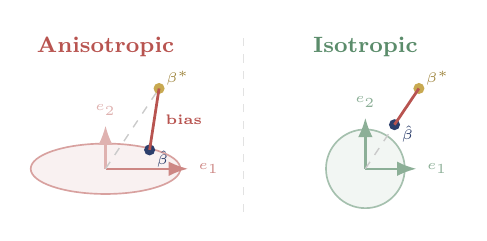
\begin{tikzpicture}[>=Latex, font=\small]
  %% ── Anisotropic panel ──
  \node[mbad, font=\footnotesize\bfseries] at (1.1,1.55) {Anisotropic};
  \draw[mbad!55, fill=mbad!8, line width=0.6pt] (1.1,0) ellipse (0.95 and 0.32);
  \draw[->, mbad!70, line width=0.9pt] (1.1,0) -- (2.15,0)  node[right, font=\tiny]{$e_1$};
  \draw[->, mbad!45, line width=0.9pt] (1.1,0) -- (1.1,0.55) node[above, font=\tiny]{$e_2$};
  \draw[mgray!55, dashed, line width=0.5pt] (1.1,0) -- (1.78,1.02);
  \fill[maccent] (1.78,1.02) circle (2pt);
  \node[maccent!80!black, font=\tiny\bfseries, above right=-2.5pt and -1pt] at (1.78,1.02) {$\beta^{*}$};
  \fill[mprimary] (1.66,0.24) circle (2pt);
  \node[mprimary, font=\tiny\bfseries, below right=-3pt and -1pt] at (1.66,0.24) {$\hat\beta$};
  \draw[mbad, line width=1pt] (1.78,1.02) -- (1.66,0.24);
  \node[mbad, font=\tiny\bfseries, right=0pt] at (1.74,0.62) {bias};

  %% ── divider ──
  \draw[mgray!30, dashed] (2.85,-0.55) -- (2.85,1.72);

  %% ── Isotropic panel ──
  \node[mgood, font=\footnotesize\bfseries] at (4.4,1.55) {Isotropic};
  \draw[mgood!55, fill=mgood!8, line width=0.6pt] (4.4,0) circle (0.5);
  \draw[->, mgood!70, line width=0.9pt] (4.4,0) -- (5.05,0)  node[right, font=\tiny]{$e_1$};
  \draw[->, mgood!70, line width=0.9pt] (4.4,0) -- (4.4,0.65) node[above, font=\tiny]{$e_2$};
  \draw[mgray!55, dashed, line width=0.5pt] (4.4,0) -- (5.08,1.02);
  \fill[maccent] (5.08,1.02) circle (2pt);
  \node[maccent!80!black, font=\tiny\bfseries, above right=-2.5pt and -1pt] at (5.08,1.02) {$\beta^{*}$};
  \fill[mprimary] (4.77,0.56) circle (2pt);
  \node[mprimary, font=\tiny\bfseries, below right=-3pt and -1pt] at (4.77,0.56) {$\hat\beta$};
  \draw[mbad, line width=1pt] (5.08,1.02) -- (4.77,0.56);
\end{tikzpicture}
}
\end{center}

\vspace{0.4em}
% ── nội dung bảng cũ: 2 chú thích màu xếp ngay dưới 2 panel ──
\begin{center}
\begin{minipage}{0.56\textwidth}
\begin{minipage}[t]{0.49\linewidth}\centering
  {\footnotesize\color{mbad}$\lambda_{\min}\ll\bar\lambda$: hướng yếu bị co mạnh\\[2pt]
   $\Rightarrow$ bias $\dfrac{\lambda}{\lambda_{\min}+\lambda}$ \textbf{cao hơn}}
\end{minipage}\hfill
\begin{minipage}[t]{0.49\linewidth}\centering
  {\footnotesize\color{mgood}$\lambda_k=\bar\lambda$: co đều mọi hướng\\[2pt]
   $\Rightarrow$ bias $\dfrac{\lambda}{\bar\lambda+\lambda}$ \textbf{thấp nhất}}
\end{minipage}
\end{minipage}
\end{center}

\vspace{0.6em}
\begin{center}
\begin{minipage}{0.84\textwidth}
\begin{primarybox}
\footnotesize\textbf{Bổ đề 1.} Với $\lambda>0$, $\exists\,\mathbf{y}$ sao cho
$\|\mathrm{Bias}(\hat\beta_{\rm aniso})\| > \|\mathrm{Bias}(\hat\beta_{\rm iso})\|$.
\end{primarybox}
\end{minipage}
\end{center}

\end{frame}


% ─── [BATCH 1] Lemma 2: Variance ─────────────────────────────────────────────
% Hero mới: "quạt decision boundary" — mỗi resample → 1 boundary; aniso xòe
% rộng (var cao), iso bó chặt (var thấp). Bố cục GƯƠNG với Bổ đề 1: text/bảng
% TRÁI, hero PHẢI.
\begin{frame}{Bổ đề 2 — Anisotropy Làm Tăng Variance}
\begin{center}
\resizebox{0.48\linewidth}{!}{%
\begin{tikzpicture}[font=\small]
  %% ── Anisotropic: quạt xòe rộng ──
  \node[mbad, font=\footnotesize\bfseries] at (1.0,1.7) {Anisotropic};
  \coordinate (PA) at (1.0,0.05);
  \fill[mbad!10] ($(PA)+(32:1.3)$) -- (PA) -- ($(PA)+(-32:1.3)$) -- cycle;
  \fill[mbad!10] ($(PA)+(148:1.3)$) -- (PA) -- ($(PA)+(212:1.3)$) -- cycle;
  \foreach \a in {-30,-20,-10,10,20,30}{
    \draw[mbad!55, line width=0.5pt] ($(PA)+(\a+180:1.3)$) -- ($(PA)+(\a:1.3)$);
  }
  \draw[mbad, line width=1.2pt] ($(PA)+(180:1.3)$) -- ($(PA)+(0:1.3)$);
  \node[mbad, font=\tiny\bfseries] at (1.0,-1.15) {var $\uparrow$ (xòe rộng)};

  %% ── divider ──
  \draw[mgray!30, dashed] (2.8,-1.35) -- (2.8,1.85);

  %% ── Isotropic: quạt bó chặt ──
  \node[mgood, font=\footnotesize\bfseries] at (4.6,1.7) {Isotropic};
  \coordinate (PI) at (4.6,0.05);
  \fill[mgood!10] ($(PI)+(9:1.3)$) -- (PI) -- ($(PI)+(-9:1.3)$) -- cycle;
  \fill[mgood!10] ($(PI)+(171:1.3)$) -- (PI) -- ($(PI)+(189:1.3)$) -- cycle;
  \foreach \a in {-8,-5,-2,2,5,8}{
    \draw[mgood!55, line width=0.5pt] ($(PI)+(\a+180:1.3)$) -- ($(PI)+(\a:1.3)$);
  }
  \draw[mgood, line width=1.2pt] ($(PI)+(180:1.3)$) -- ($(PI)+(0:1.3)$);
  \node[mgood!70!black, font=\tiny\bfseries] at (4.6,-1.15) {var $\downarrow$ (bó chặt)};
\end{tikzpicture}
}
\end{center}

\vspace{0.1em}
\begin{center}{\scriptsize\color{mgray} Mỗi đường $=$ một decision boundary từ một lần resample.}\end{center}

\vspace{0.2em}
% ── nội dung bảng cũ: 2 chú thích màu xếp ngay dưới 2 panel ──
\begin{center}
\begin{minipage}{0.56\textwidth}
\begin{minipage}[t]{0.49\linewidth}\centering
  {\footnotesize\color{mbad}$\lambda_k$ không đều\\[2pt]$\Rightarrow$ boundary \textbf{dao động}}
\end{minipage}\hfill
\begin{minipage}[t]{0.49\linewidth}\centering
  {\footnotesize\color{mgood}$\lambda_k=\bar\lambda$\\[2pt]$\Rightarrow$ boundary \textbf{ổn định}}
\end{minipage}
\end{minipage}
\end{center}

\vspace{0.6em}
\begin{center}
\begin{minipage}{0.84\textwidth}
\begin{primarybox}
\footnotesize\textbf{Bổ đề 2.} Với $\lambda=0$:\;
$\mathrm{tr}(\mathrm{Var}(\hat\beta_{\rm aniso})) > \mathrm{tr}(\mathrm{Var}(\hat\beta_{\rm iso}))$;
đẳng thức $\Leftrightarrow$ mọi trị riêng bằng nhau.
\end{primarybox}
\end{minipage}
\end{center}

\end{frame}


% ─── [BATCH 1] Định lý 1 — synthesis của 2 bổ đề ─────────────────────────────
% Synthesis: [Bổ đề 1 ⊕ Bổ đề 2] ⇒ proof pipeline (Cramér–Rao → Jensen) ⇒
% công thức hero N(0, κ/K·I).
\begin{frame}{Định lý 1 — Isotropic Gaussian Là Điểm Cực Tiểu Duy Nhất}

% ── Synthesis + proof pipeline ───────────────────────────────────────────────
\begin{center}
\resizebox{\linewidth}{!}{%
\begin{tikzpicture}[>=Latex, every node/.style={font=\small}]

  % Hai bổ đề gộp lại
  \node[rbox, font=\scriptsize, align=center, minimum width=1.9cm, minimum height=0.85cm] (bd1) at (0,0.62)
    {\textbf{Bổ đề 1}\\ Bias $\uparrow$};
  \node[rbox, font=\scriptsize, align=center, minimum width=1.9cm, minimum height=0.85cm] (bd2) at (0,-0.62)
    {\textbf{Bổ đề 2}\\ Var $\uparrow$};
  \node[font=\large\bfseries, mprimary] (op) at (1.55,0) {$\oplus$};
  \draw[arr] (bd1.east) to[out=0,in=120] (op);
  \draw[arr] (bd2.east) to[out=0,in=240] (op);

  % Pipeline
  \node[pbox, align=center, font=\scriptsize, minimum width=2.15cm, minimum height=1.0cm] (p0) at (3.4,0)
    {Phân phối bất kỳ $p$\\[2pt]$\mathrm{Tr}(\mathrm{Cov})=\kappa$};
  \node[pbox, align=center, font=\scriptsize, minimum width=1.8cm, minimum height=1.0cm] (p1) at (7.2,0)
    {$\mathcal{N}(0,\Sigma)$\\[2pt]$\Sigma$ bất kỳ};
  \node[gbox, draw=mgood!80, line width=1.2pt, align=center, font=\scriptsize,
        minimum width=2.5cm, minimum height=1.0cm] (p2) at (10.9,0)
    {$p^{*}=\mathcal{N}\!\left(0,\tfrac{\kappa}{K}I\right)$\\[2pt]\textbf{Isotropic}};

  \draw[arr, line width=1pt] (op) -- (p0.west);
  \draw[arr, line width=1pt] (p0.east) -- (p1.west)
    node[above=1pt, midway, font=\tiny, mprimary]{\textbf{Cramér–Rao}};
  \draw[arr, line width=1pt] (p1.east) -- (p2.west)
    node[above=1pt, midway, font=\tiny, mprimary]{\textbf{Jensen}};

  \node[mgood, font=\tiny\bfseries, above=5pt of p2] {$\checkmark$\;cực tiểu duy nhất};
\end{tikzpicture}
}
\end{center}

% ── Hero formula ─────────────────────────────────────────────────────────────
\vspace{0.4em}
\begin{center}
{\LARGE\bfseries\color{mprimary}$f_\theta(\mathbf{x}) \sim \mathcal{N}\!\left(\mathbf{0},\,\tfrac{\kappa}{K} I\right)$}%
\hspace{0.8em}{\normalsize\color{mgood!55!black}— điểm cực tiểu \textbf{duy nhất}}
\end{center}

\vspace{0.5em}
\begin{center}
\begin{minipage}{0.9\textwidth}
\begin{accentbox}
\footnotesize\textbf{Định lý 1} (Balestriero \& LeCun, 2025): đúng cho \textbf{mọi} probe family — linear probe, kNN, kernel regression. Không phân phối nào khác đạt minimum này; \textbf{target duy nhất} của encoder, không cần heuristic.
\end{accentbox}
\end{minipage}
\end{center}

\takeaway{$f_\theta(\mathbf{x}) \sim \mathcal{N}(\mathbf{0}, I)$ là \emph{duy nhất} tối ưu cho mọi downstream task}

\end{frame}


% ─── [BATCH 1] Theory summary ────────────────────────────────────────────────
\begin{frame}{Kết Luận Lý Thuyết: Design Principle Cho LeJEPA}

\vfill
\begin{center}
  {\footnotesize\color{mgray}\itshape Định lý 1 (Balestriero \& LeCun, 2025) suy ra:}\\[14pt]

  {\Huge\bfseries\color{mprimary}
  $f_\theta(\mathbf{x}) \;\sim\; \mathcal{N}(\mathbf{0},\, I)$}\\[16pt]

  {\normalsize\color{mgray} Đây là design principle \textbf{duy nhất} cần đạt}
\end{center}
\vfill

\begin{columns}[t]
\column{0.32\textwidth}
  \centering\footnotesize
  \textcolor{mgood}{\textbf{\checkmark}}\;\textbf{Linear probe}\\tối ưu (bias + var)
\column{0.32\textwidth}
  \centering\footnotesize
  \textcolor{mgood}{\textbf{\checkmark}}\;\textbf{kNN probe}\\tối ưu (ISB)
\column{0.32\textwidth}
  \centering\footnotesize
  \textcolor{mgood}{\textbf{\checkmark}}\;\textbf{Kernel probe}\\tối ưu (ISB)
\end{columns}
\vfill

\takeaway{Lần đầu: biết \textbf{chính xác} embeddings nên phân phối thế nào — giờ cần công cụ để đến đó}

\end{frame}


% ─── Slide 6: Why sphere — geometric ─────────────────────────────────────────
% Minh họa aniso-ellipsoid vs iso-sphere, có thêm khung "kNN neighborhood" so
% với slide "Phân phối Nào Là Tối Ưu" — giữ lại vì đào sâu trực giác kNN.
% [ĐÃ TẮT] commented-out theo yêu cầu — trùng trực giác aniso→iso với các slide trước.
\iffalse
\begin{frame}{Tại Sao Hình Cầu: Biến Đổi Không Gian Latent}

\begin{center}
\begin{tikzpicture}[scale=0.95, every node/.style={font=\small}]

  %% ── Style definitions ──
  \tikzset{
    querynode/.style={fill=mprimary, draw=white, line width=0.6pt,
                      circle, inner sep=0, minimum size=7pt},
    notelabel/.style={draw=mgray!50, fill=mlight, rounded corners=3pt,
                      font=\scriptsize\itshape, inner sep=4pt, text=mdark!90},
  }

  %% ═══════════ LEFT: Anisotropic ═══════════
  \node[mbad, font=\small\bfseries] at (1.5, 3.55) {Anisotropic};

  %% Density contours (4 concentric ellipses, fading outward)
  \fill[mbad!22, opacity=0.75] (1.5, 1.85) ellipse (1.95cm and 0.60cm);
  \fill[mbad!35, opacity=0.75] (1.5, 1.85) ellipse (1.40cm and 0.42cm);
  \fill[mbad!52, opacity=0.75] (1.5, 1.85) ellipse (0.88cm and 0.25cm);
  \fill[mbad!68, opacity=0.75] (1.5, 1.85) ellipse (0.42cm and 0.12cm);
  %% Contour outlines
  \draw[mbad!50, line width=0.55pt] (1.5, 1.85) ellipse (1.95cm and 0.60cm);
  \draw[mbad!65, line width=0.55pt] (1.5, 1.85) ellipse (1.40cm and 0.42cm);
  \draw[mbad!82, line width=0.65pt] (1.5, 1.85) ellipse (0.88cm and 0.25cm);

  %% kNN neighborhood — distorted ellipse
  \draw[mprimary!65, dashed, line width=1.2pt] (1.5, 1.85) ellipse (0.98cm and 0.40cm);

  %% Scatter points — refined flat dots
  \foreach \x/\y in {-1.40/0.00, -0.90/0.05, -0.35/-0.08, 0.20/0.09,
                      0.65/-0.04, 1.10/0.06, 1.30/0.01}{
    \filldraw[fill=mbad!80, draw=white, line width=0.3pt, opacity=0.95]
      ({1.5+\x},{1.85+\y}) circle (1.5pt);
  }

  %% Query point q
  \node[querynode] at (1.5, 1.85) {};
  \node[mprimary!90, font=\scriptsize\bfseries, above right=-0.5pt and 2pt]
    at (1.5, 1.85) {$q$};

  %% Eigenvalue axes
  \draw[->, mbad!90, line width=1.3pt]  (1.5,1.85) -- (3.15,1.85)
    node[right=-1pt, font=\tiny\bfseries]{$e_1$};
  \draw[->, mbad!55, line width=1.0pt]  (1.5,1.85) -- (1.5, 2.55)
    node[above=-1pt, font=\tiny\bfseries]{$e_2$};

  %% λ annotation inline
  \node[mbad, font=\tiny\bfseries, align=center, fill=white, inner sep=1.5pt, rounded corners=2pt, fill opacity=0.8, text opacity=1] at (2.6, 2.6)
    {$\lambda_1 \gg \lambda_2$};

  %% Note label — kNN skewed
  \node[notelabel] at (1.5, -0.05)
    {kNN neighborhood bị kéo lệch};
  \node[mbad!85, font=\scriptsize\bfseries, align=center] at (1.5, -0.6)
    {bias$\;\uparrow$\quad var$\;\uparrow$};


  %% ═══════════ ARROW ═══════════
  \draw[->, thick, mprimary] (3.6, 1.85) -- (4.55, 1.85)
    node[above=2pt, midway, font=\footnotesize\bfseries]{\textbf{SIGReg}}
    node[below=1pt, midway, font=\tiny]{$\Sigma \xrightarrow{\;\mathcal{L}\;} I$};


  %% ═══════════ RIGHT: Isotropic ═══════════
  \node[mgood, font=\small\bfseries] at (6.4, 3.55)
    {Isotropic $\mathcal{N}(0,I)$};

  %% Density contours (4 concentric circles, fading outward)
  \fill[mgood!22, opacity=0.75] (6.4, 1.85) circle (1.12cm);
  \fill[mgood!35, opacity=0.75] (6.4, 1.85) circle (0.80cm);
  \fill[mgood!52, opacity=0.75] (6.4, 1.85) circle (0.50cm);
  \fill[mgood!68, opacity=0.75] (6.4, 1.85) circle (0.22cm);
  %% Contour outlines
  \draw[mgood!50, line width=0.55pt] (6.4, 1.85) circle (1.12cm);
  \draw[mgood!65, line width=0.55pt] (6.4, 1.85) circle (0.80cm);
  \draw[mgood!82, line width=0.65pt] (6.4, 1.85) circle (0.50cm);

  %% kNN neighborhood — symmetric circle
  \draw[mprimary!65, dashed, line width=1.2pt] (6.4, 1.85) circle (0.54cm);

  %% Scatter points — refined flat dots
  \foreach \ang in {0,60,120,180,240,300}{
    \filldraw[fill=mgood!80, draw=white, line width=0.3pt, opacity=0.95]
      ({6.4+0.90*cos(\ang)},{1.85+0.90*sin(\ang)}) circle (1.5pt);
  }

  %% Query point q
  \node[querynode] at (6.4, 1.85) {};
  \node[mprimary!90, font=\scriptsize\bfseries, above right=-0.5pt and 2pt]
    at (6.4, 1.85) {$q$};

  %% Three equal axes
  \draw[->, mgood!88, line width=1.2pt] (6.4,1.85) -- (7.60,1.85)
    node[right=-1pt, font=\tiny\bfseries]{$e_1$};
  \draw[->, mgood!88, line width=1.2pt] (6.4,1.85) -- (6.4,3.05)
    node[above=-1pt, font=\tiny\bfseries]{$e_2$};
  \draw[->, mgood!88, line width=1.2pt] (6.4,1.85) --
    ({6.4-0.72},{1.85-0.72})
    node[below left=-1pt, font=\tiny\bfseries]{$e_3$};

  %% λ = 1 annotation inline
  \node[mgood, font=\tiny\bfseries, align=left, fill=white, inner sep=1.5pt, rounded corners=2pt, fill opacity=0.8, text opacity=1, anchor=west] at (7.2, 2.8)
    {$\lambda_1{=}\lambda_2{=}1$};

  %% Note label — kNN uniform
  \node[notelabel] at (6.4, -0.05)
    {kNN neighborhood đồng đều};
  \node[mgood!85, font=\scriptsize\bfseries, align=center] at (6.4, -0.6)
    {bias$\;\downarrow$\quad var$\;\downarrow$};

\end{tikzpicture}
\end{center}

\end{frame}
\fi


% ─── [BATCH 2] High-dim challenge ────────────────────────────────────────────
% ─── Frame: Hypothesis Testing as a Judge ─────────────────────────────────────
\begin{frame}{Ý Tưởng: Dùng Statistical Test Như Một Hàm Loss}

\vspace{0.3em}
\textbf{Mục tiêu:} ép $P_\theta$ (phân phối của embedding) về $Q = \mathcal{N}(0,I)$.

\vspace{0.5em}
Thay vì đo khoảng cách trực tiếp (tốn kém), ta frame lại thành:

\vspace{0.3em}
\begin{accentbox}
\[
  H_0 : P_\theta = Q \qquad \text{vs} \qquad H_1 : P_\theta \neq Q
\]
\centering\footnotesize
Test statistic $T$ đo lường \textbf{bằng chứng thực nghiệm chống lại} $H_0$.
\end{accentbox}

\vspace{0.8em}
\begin{columns}[T]
\column{0.48\textwidth}

\begin{center}
\begin{tikzpicture}[every node/.style={font=\scriptsize}, scale=0.90]
  \draw[->, thick, mgray!60] (-0.3,0) -- (6.2,0)
    node[right, font=\tiny, mgray]{$T$};

  \fill[mgood!15] (0,0.05) rectangle (3.2,0.75);
  \draw[mprimary, dashed, thick] (3.2,-0.1) -- (3.2,0.85)
    node[above, mprimary, font=\tiny\bfseries]{$\tau_\alpha$};

  \fill[mbad!12] (3.2,0.05) rectangle (6.0,0.75);

  \node[mgood, font=\tiny\bfseries, align=center] at (1.6, 0.38)
    {$T$ nhỏ\\embedding $\approx$ Gaussian};
  \node[mbad, font=\tiny\bfseries, align=center] at (4.7, 0.38)
    {$T$ lớn\\embedding xa Gaussian};

  \draw[->, very thick, mprimary] (4.8,-0.55) -- (1.5,-0.55)
    node[midway, below=2pt, font=\tiny\bfseries, mprimary]
      {$\Rightarrow$ \textbf{Minimize} $T$ như một loss};
\end{tikzpicture}
\end{center}

\column{0.48\textwidth}

\begin{goodbox}
\footnotesize \textbf{Câu hỏi tiếp theo:}\\[4pt]
Chọn test $T$ nào?\\[4pt]
Cần $T$ vừa \textbf{differentiable}, vừa \textbf{scalable}, vừa \textbf{provably correct} — ba họ test sẽ được xét lần lượt.
\end{goodbox}

\end{columns}

\takeaway{Minimize $T$ = thu thập ít bằng chứng chống lại $H_0$ = ép embedding về $\mathcal{N}(0,I)$}

\end{frame}


\begin{frame}{Thách Thức: Kiểm Tra Phân Phối Trong Không Gian Cao Chiều}

\vspace{1em}
\begin{center}
\renewcommand{\arraystretch}{1.8}
\begin{tabular}{@{} l c c c @{}}
\toprule
\textbf{Phương pháp} & \textbf{Differentiable} & \textbf{Scalable} $\mathcal{O}(N)$ & \textbf{Provably Correct} \\
\midrule
\textbf{MMD} & \textcolor{mgood}{\cmark} & \textcolor{mbad}{\xmark} \footnotesize ($\mathcal{O}(N^2)$) & \textcolor{mgood}{\cmark} \\
\textbf{KL Divergence} & \textcolor{mbad}{\xmark} \footnotesize (unstable) & \textcolor{mgood}{\cmark} & \textcolor{mgood}{\cmark} \\
\textbf{Test chuẩn (BHEP, Mardia)} & \textcolor{mgood}{\cmark} & \textcolor{mbad}{\xmark} \footnotesize ($\mathcal{O}(N^2)$) & \textcolor{mgood}{\cmark} \\
\midrule
\rowcolor{mgood!15}
\textbf{SIGReg} & \textcolor{mgood}{\textbf{\cmark}} & \textcolor{mgood}{\textbf{\cmark}} & \textcolor{mgood}{\textbf{\cmark}} \\
\bottomrule
\end{tabular}
\end{center}

\vspace{1.5em}
\begin{accentbox}
\footnotesize \textbf{Giải pháp SIGReg:} Phân rã bài toán $K$-chiều thành $M$ bài toán 1D độc lập qua \textbf{random projection} (Cramér-Wold), giúp đạt được cả 3 tiêu chí!
\end{accentbox}

\end{frame}


% ─── [BATCH 2] 3 families — Moments unstable ─────────────────────────────────
\begin{frame}{Họ Test 1: Moments — Mạnh Nhưng Gradient Explode}

\vspace{2.5em}
\begin{center}
\begin{tikzpicture}
\begin{axis}[
  width=12cm, height=5.5cm,
  xlabel={Moment order $K$},
  ylabel={$\|\nabla_z \mathcal{L}_K\|$},
  xmin=1, xmax=6.2, ymin=0, ymax=140,
  grid=none,
  axis x line=bottom, axis y line=left,
  clip=false,
  xtick={1,2,3,4,5,6},
  ytick=\empty,
]
  % Vùng rủi ro (Unstable Region) dịch sang 4.2
  \fill[mbad!10] (axis cs:4.2,0) rectangle (axis cs:6.2,140);
  \draw[mbad, dashed, thick] (axis cs:4.2,0) -- (axis cs:4.2,140);
  
  % Đường cong chia 2 màu (an toàn vs nổ)
  \addplot[mprimary, ultra thick, domain=1:4.2, samples=20] {2.5^x};
  \addplot[mbad, ultra thick, domain=4.2:5.38, samples=20] {2.5^x};
  
  % Chú thích
  \node[mprimary, align=center] at (axis cs:2.5, 40) {
    \small\bfseries Shortcut\\[0.2em]
    \footnotesize (Định lý 3)
  };
  
  % Chú thích Vùng Unstable
  \node[mbad, align=center] at (axis cs:5.3, 40) {
    \large\bfseries VÙNG UNSTABLE\\[0.4em]
    \small \textbf{Gradient Explode}\\[0.1em]
    \small (Hàm mũ)
  };
  
  % EJB callout (không dùng mũi tên)
  \node[align=center, fill=mlight, draw=mgray!50, rounded corners, font=\footnotesize] (ejb) at (axis cs:2.5, 90) {
    \textbf{Extended Jarque-Bera (EJB)}\\
    Gom 4 moments ($K=4$)
  };
  
\end{axis}
\end{tikzpicture}
\end{center}

\vspace{1.5em}
\begin{badbox}
\footnotesize \textbf{Kết luận:} Sự tiến thoái lưỡng nan: Tăng $K$ để vá lỗi shortcut sẽ trực tiếp đẩy mô hình vào vùng Gradient Explode.
\end{badbox}

\end{frame}


% ─── [BATCH 2] CDF family ────────────────────────────────────────────────────
\begin{frame}{Họ Test 2: CDF — Chính Xác Nhưng Không Differentiable}

\vspace{0.4em}
Họ test CDF đo khoảng cách giữa hai hàm phân bố tích luỹ. Thao tác \textbf{sắp xếp} (sort) dữ liệu tạo ra 2 nút thắt chí mạng:

\vspace{1.2em}
\begin{columns}[T]
\column{0.48\textwidth}
\begin{center}
\textcolor{mbad}{\textbf{\large Vấn đề 1: Non-parallel}}

\vspace{0.8em}
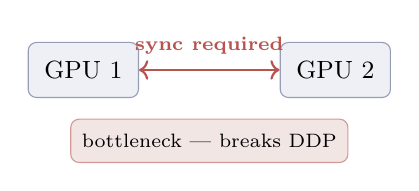
\begin{tikzpicture}[every node/.style={font=\scriptsize}]
  \node[pbox, minimum width=1.4cm, minimum height=0.7cm, font=\small]
    (g1) at (0, 0) {GPU 1};
  \node[pbox, minimum width=1.4cm, minimum height=0.7cm, font=\small]
    (g2) at (3.2, 0) {GPU 2};
  \draw[<->, thick, mbad] (g1.east) -- (g2.west)
    node[midway, above=2pt, font=\scriptsize\bfseries, mbad]{sync required};
  \node[rbox, minimum width=3.4cm, minimum height=0.55cm, font=\scriptsize, inner sep=4pt]
    at (1.6, -0.9) {bottleneck — breaks DDP};
\end{tikzpicture}
\end{center}

\column{0.48\textwidth}
\begin{center}
\textcolor{mbad}{\textbf{\large Vấn đề 2: Non-differentiable}}

\vspace{0.8em}
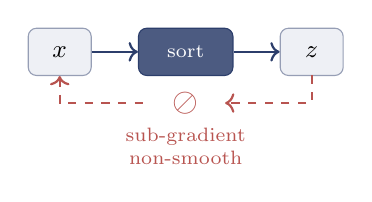
\begin{tikzpicture}[every node/.style={font=\scriptsize}]
  \node[pbox, minimum width=0.8cm, minimum height=0.6cm] (xn) at (0,0) {$x$};
  \node[darkbox, minimum width=1.2cm, minimum height=0.6cm, font=\scriptsize]
    (srt) at (1.6,0) {sort};
  \node[pbox, minimum width=0.8cm, minimum height=0.6cm] (zn) at (3.2,0) {$z$};
  \draw[arr] (xn)--(srt);
  \draw[arr] (srt)--(zn);
  
  \draw[<-, dashed, mbad, thick] (xn.south) -- (0,-0.65) -- (1.1,-0.65);
  \node[mbad, font=\large\bfseries] at (1.6,-0.65) {$\oslash$};
  \draw[->, dashed, mbad, thick] (3.2,-0.3) -- (3.2,-0.65) -- (2.1,-0.65);
  \node[mbad, font=\scriptsize, align=center] at (1.6,-1.2)
    {sub-gradient\\non-smooth};
\end{tikzpicture}
\end{center}
\end{columns}

\vspace{1.5em}
\takeaway{Hạn chế cốt lõi của CDF: Phép toán sắp xếp bẻ gãy tính toán song song và triệt tiêu luồng gradient}
\end{frame}


% ─── [BATCH 2] Epps-Pulley (ECF) ─────────────────────────────────────────────
\begin{frame}{Họ Test 3: ECF — Stable, Scalable, Provable}

\vfill
% Công thức làm caption
\begin{center}\small
$\displaystyle \hat{\phi}_X(t) = \frac{1}{N}\sum_{n=1}^N e^{it X_n}$
\qquad
$\displaystyle EP = \int_{-\infty}^{\infty}
   \bigl| \hat{\phi}_X(t) - \phi_{\mathcal{N}}(t) \bigr|^2 w(t)\,dt$
\end{center}

\vspace{0.3em}
% Plot hero — chú giải trực tiếp
\begin{center}
\begin{tikzpicture}
\begin{axis}[
  width=11cm, height=4.6cm,
  xlabel={$t$ (tần số)}, ylabel={CF},
  xlabel style={font=\small}, ylabel style={font=\small},
  tick label style={font=\tiny},
  xmin=-5, xmax=5, ymin=-0.3, ymax=1.25,
  grid=major, grid style={mgray!15},
  clip=false, no marks,
]
  % vùng gap = EP (nền)
  \addplot[fill=mbad!12, draw=none, domain=-3.5:3.5, samples=80]
    {exp(-x^2/2) + 0.22*sin(deg(3.5*x))*exp(-x^2/2.2) + 0.08*cos(deg(7*x))*exp(-x^2/3)}
    \closedcycle;
  \addplot[fill=white, draw=none, domain=-3.5:3.5, samples=80]
    {exp(-x^2/2)} \closedcycle;
  % hai đường
  \addplot[mprimary, very thick, domain=-5:5, samples=60] {exp(-x^2/2)};
  \addplot[maccent, thick, domain=-5:5, samples=80]
    {exp(-x^2/2) + 0.22*sin(deg(3.5*x))*exp(-x^2/2.2) + 0.08*cos(deg(7*x))*exp(-x^2/3)};
  % chú giải trực tiếp
  \node[font=\footnotesize, mprimary, anchor=east] at (axis cs:-1.5,1.02) {Target $\phi(t)$};
  \draw[mprimary, thin] (axis cs:-1.5,0.98) -- (axis cs:-0.55,0.86);
  \node[font=\footnotesize, maccent!80!black, anchor=west] at (axis cs:1.7,0.92) {Empirical $\hat\phi_X(t)$};
  \draw[maccent!80!black, thin] (axis cs:1.65,0.88) -- (axis cs:0.75,0.72);
  \node[font=\footnotesize\bfseries, mbad!80!black] at (axis cs:2.0,1.12) {gap $=EP$};
  \draw[mbad!70, thin] (axis cs:1.3,1.08) -- (axis cs:0.5,0.97);
\end{axis}
\end{tikzpicture}
\end{center}

\vspace{0.5em}
% 3 tính chất — chip neo dưới
\begin{center}
\begin{tikzpicture}[
    chip/.style={draw=mgood!45, fill=mlightsage, rounded corners=8pt,
                 minimum width=3.7cm, minimum height=1.4cm, align=center, inner sep=6pt}]
  \node[chip] (c1) at (0,0)    {\footnotesize\textbf{\color{mgood!55!black}Differentiable}\\[4pt] không sort $\Rightarrow \nabla$ mượt};
  \node[chip] (c2) at (4.3,0)  {\footnotesize\textbf{\color{mgood!55!black}Scalable $\mathcal{O}(N)$}\\[4pt] $\sum$ dễ \texttt{all\_reduce}};
  \node[chip] (c3) at (8.6,0)  {\footnotesize\textbf{\color{mgood!55!black}Provably Stable}\\[4pt] $|e^{itx}|=1 \Rightarrow \nabla$ bị chặn};
\end{tikzpicture}
\end{center}
\vfill
\end{frame}


% ─── Slide 7: SIGReg ─────────────────────────────────────────────────────────
\begin{frame}{Cramér-Wold: Nếu Embedding Chuẩn Thì Mọi Hình Chiếu Đều Chuẩn}

\begin{columns}[c]
\column{0.40\textwidth}

\begin{center}
\begin{tikzpicture}[
    cw/.style={rounded corners=6pt, text width=3.7cm, align=center,
               inner sep=8pt, font=\small}]
  \node[cw, draw=mprimary!55, fill=mlight] (a) at (0,2.35)
    {\textbf{Embedding}\\[3pt] $\mathbf{Z}\sim\mathcal{N}(\mathbf{0},I_K)$};
  \node[cw, draw=mgood!55, fill=mlightsage] (b) at (0,0)
    {\textbf{Mọi hình chiếu 1D}\\[3pt] $\mathbf{u}^{\top}\mathbf{Z}\sim\mathcal{N}(0,1)$};
  % chiều xuôi (hiển nhiên)
  \draw[-{Latex[length=2.6mm]}, thick, mprimary]
    ([xshift=-0.75cm]a.south) -- node[left, font=\scriptsize, mprimary] {hiển nhiên}
    ([xshift=-0.75cm]b.north);
  % chiều ngược (Cramér–Wold)
  \draw[-{Latex[length=2.6mm]}, thick, maccent!85!black]
    ([xshift=0.75cm]b.north) -- node[right, font=\scriptsize, maccent!85!black] {Cramér–Wold}
    ([xshift=0.75cm]a.south);
\end{tikzpicture}
\end{center}

\vspace{0.5em}
{\footnotesize\color{mgray}
$\mathbf{u}^{\top}\mathbf{Z}\sim\mathcal{N}(0,\mathbf{u}^{\top}I_K\mathbf{u})=\mathcal{N}(0,1)$ với $\|\mathbf{u}\|_2=1$.}

\column{0.60\textwidth}
\begin{center}
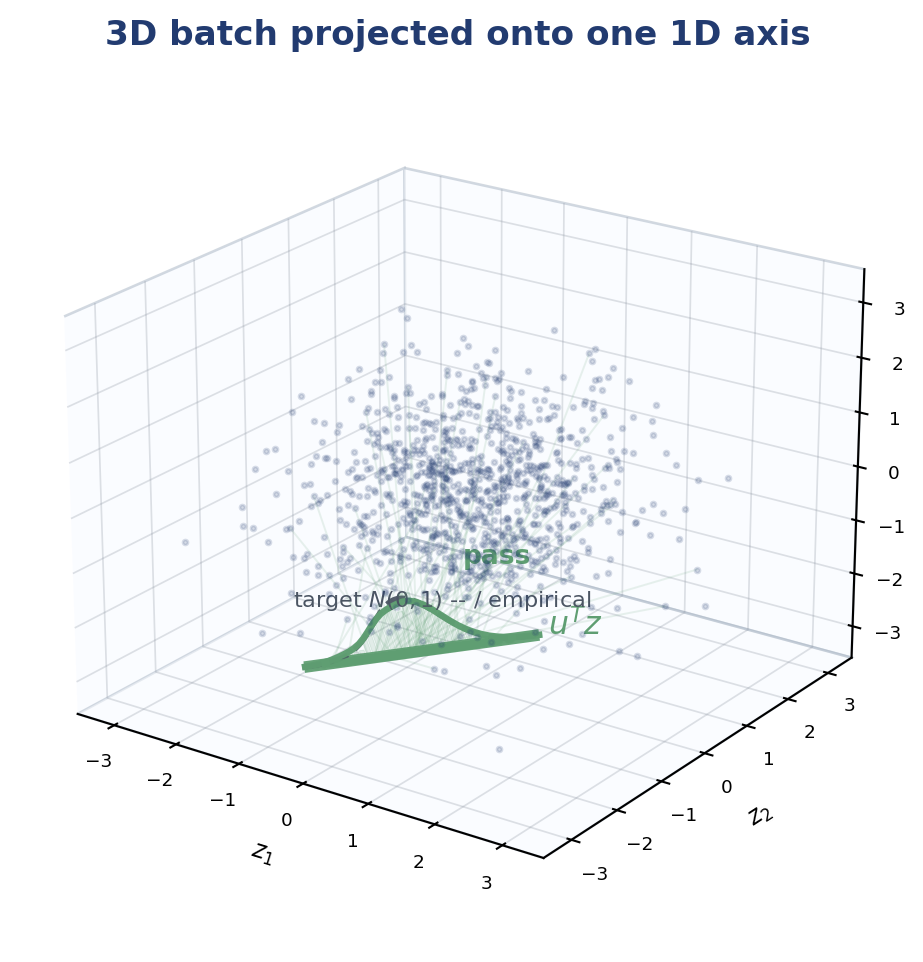
\includegraphics[width=\linewidth,height=0.60\textheight,keepaspectratio]{sigreg_gaussian_projection_line.png}
\end{center}

\vspace{-0.6em}
{\tiny\color{mgray}
\textbf{Ghi chú:} Hình mô phỏng Gaussian để trực quan hóa hình chiếu 1D; không phải kết quả thực nghiệm.
}

\end{columns}

\vspace{-0.1em}
\begin{mdframed}[
  linecolor=maccent, linewidth=1.5pt,
  backgroundcolor=mlightgold,
  innertopmargin=5pt, innerbottommargin=5pt,
  innerleftmargin=10pt, innerrightmargin=10pt,
  roundcorner=3pt, skipabove=2pt, skipbelow=0pt
]
\centering\small\bfseries\color{mprimary}
Đây là target của SIGReg: mọi projection đều phải trông như $\mathcal{N}(0,1)$,
rồi ta dùng các test 1D để kiểm điều đó trong thực tế.
\end{mdframed}

\end{frame}


\iffalse
\begin{frame}{SIGReg: Cramér-Wold Nhìn Qua Các Hình Chiếu}

\vspace{-0.65em}
\begin{center}
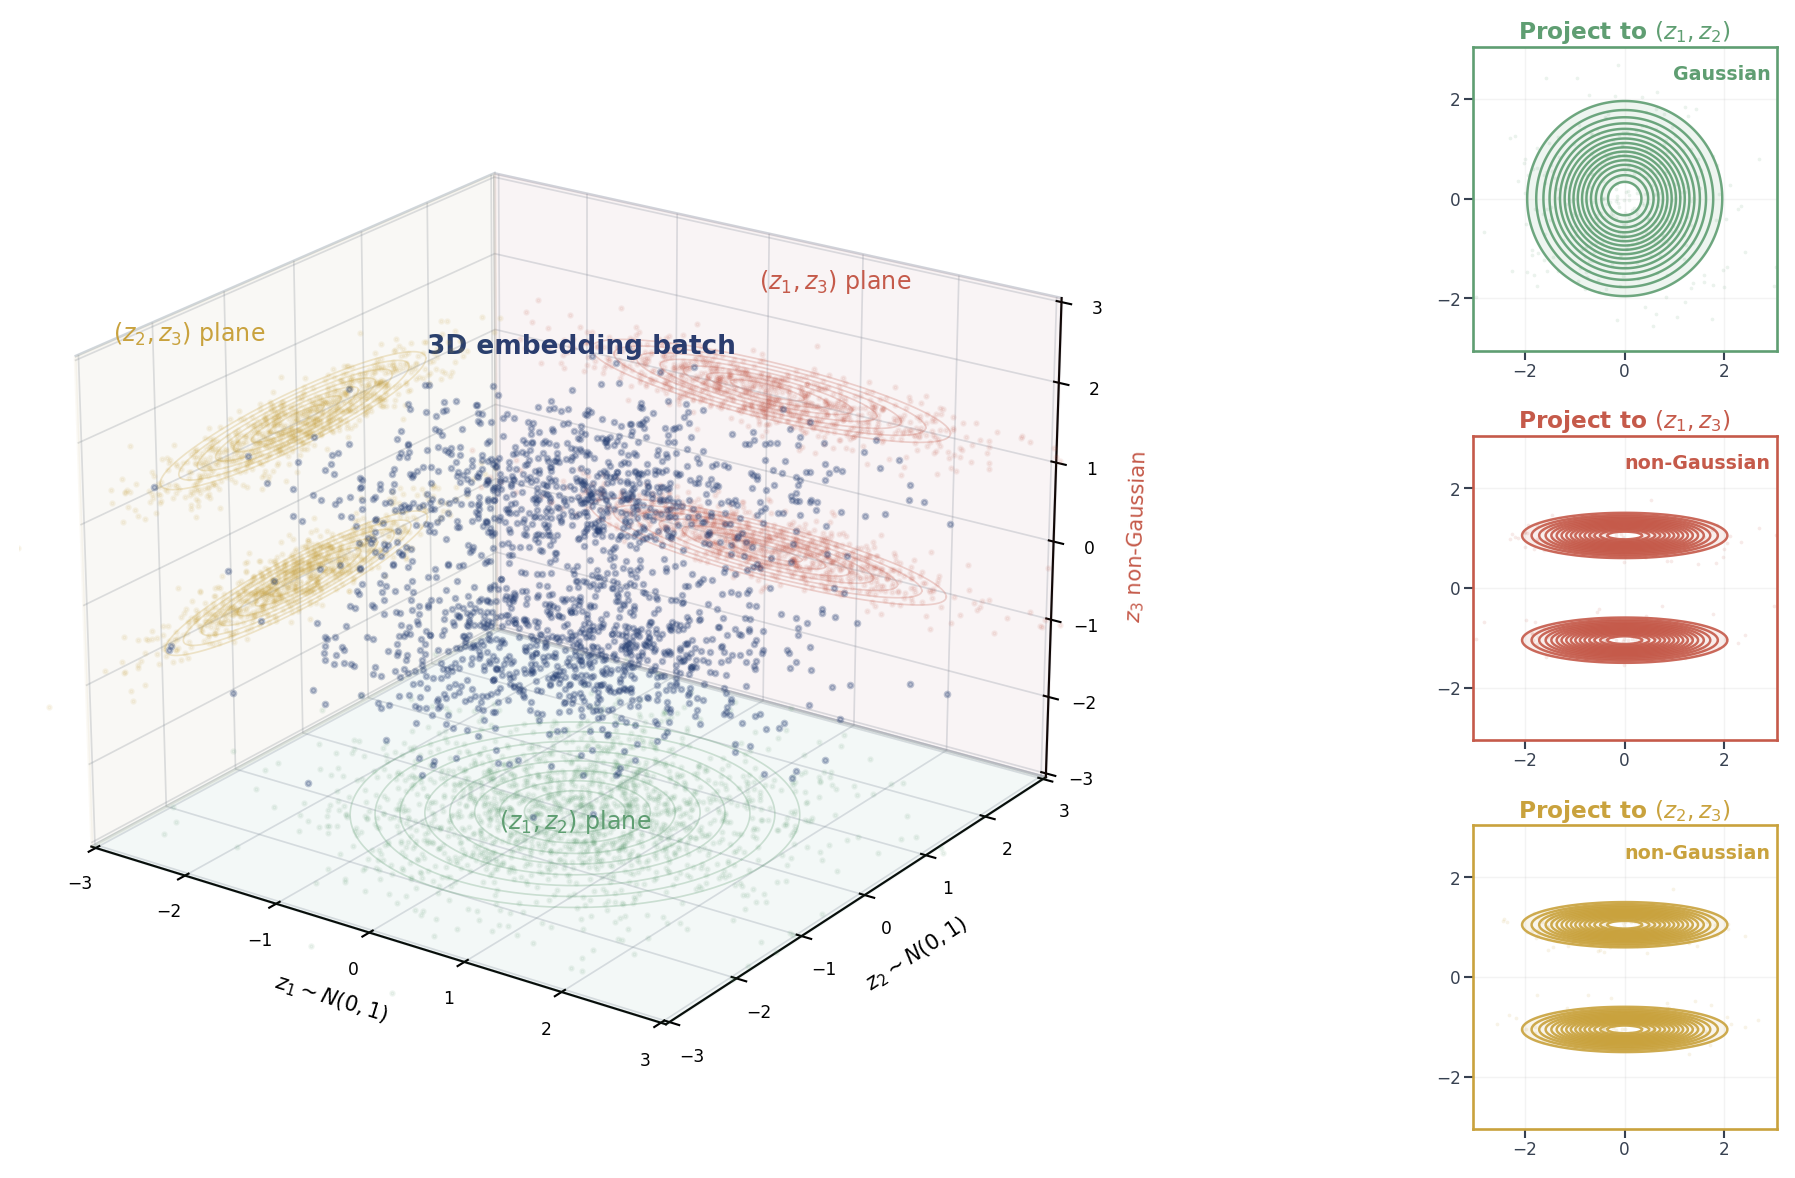
\includegraphics[width=\textwidth,height=0.71\textheight,keepaspectratio]{sigreg_projection_planes.png}
\end{center}

\vspace{-0.7em}
{\tiny\color{mgray}
\textbf{Ghi chú:} Hình tạo bằng matplotlib từ dữ liệu mô phỏng để trực quan hóa embedding và các bóng 2D. Đây là hình minh họa trực giác; Cramér-Wold/SIGReg ở slide sau dùng các hình chiếu 1D.
}

\vspace{0.15em}
\begin{mdframed}[
  linecolor=maccent, linewidth=1.5pt,
  backgroundcolor=mlightgold,
  innertopmargin=5pt, innerbottommargin=5pt,
  innerleftmargin=10pt, innerrightmargin=10pt,
  roundcorner=3pt, skipabove=2pt, skipbelow=0pt
]
\centering\small\bfseries\color{mprimary}
Bóng $(z_1,z_2)$ nhìn gần chuẩn, nhưng các bóng chứa $z_3$ lộ rõ hai cụm.\\[-1pt]
Trực giác 2D: chỉ cần có hướng nhìn thấy lệch, SIGReg sẽ phạt qua các slice 1D.
\end{mdframed}
\end{frame}
\fi


\begin{frame}{SIGReg: Slice 1D Nào Lệch Thì Slice Đó Bị Phạt}

\vspace{-0.65em}
\begin{center}
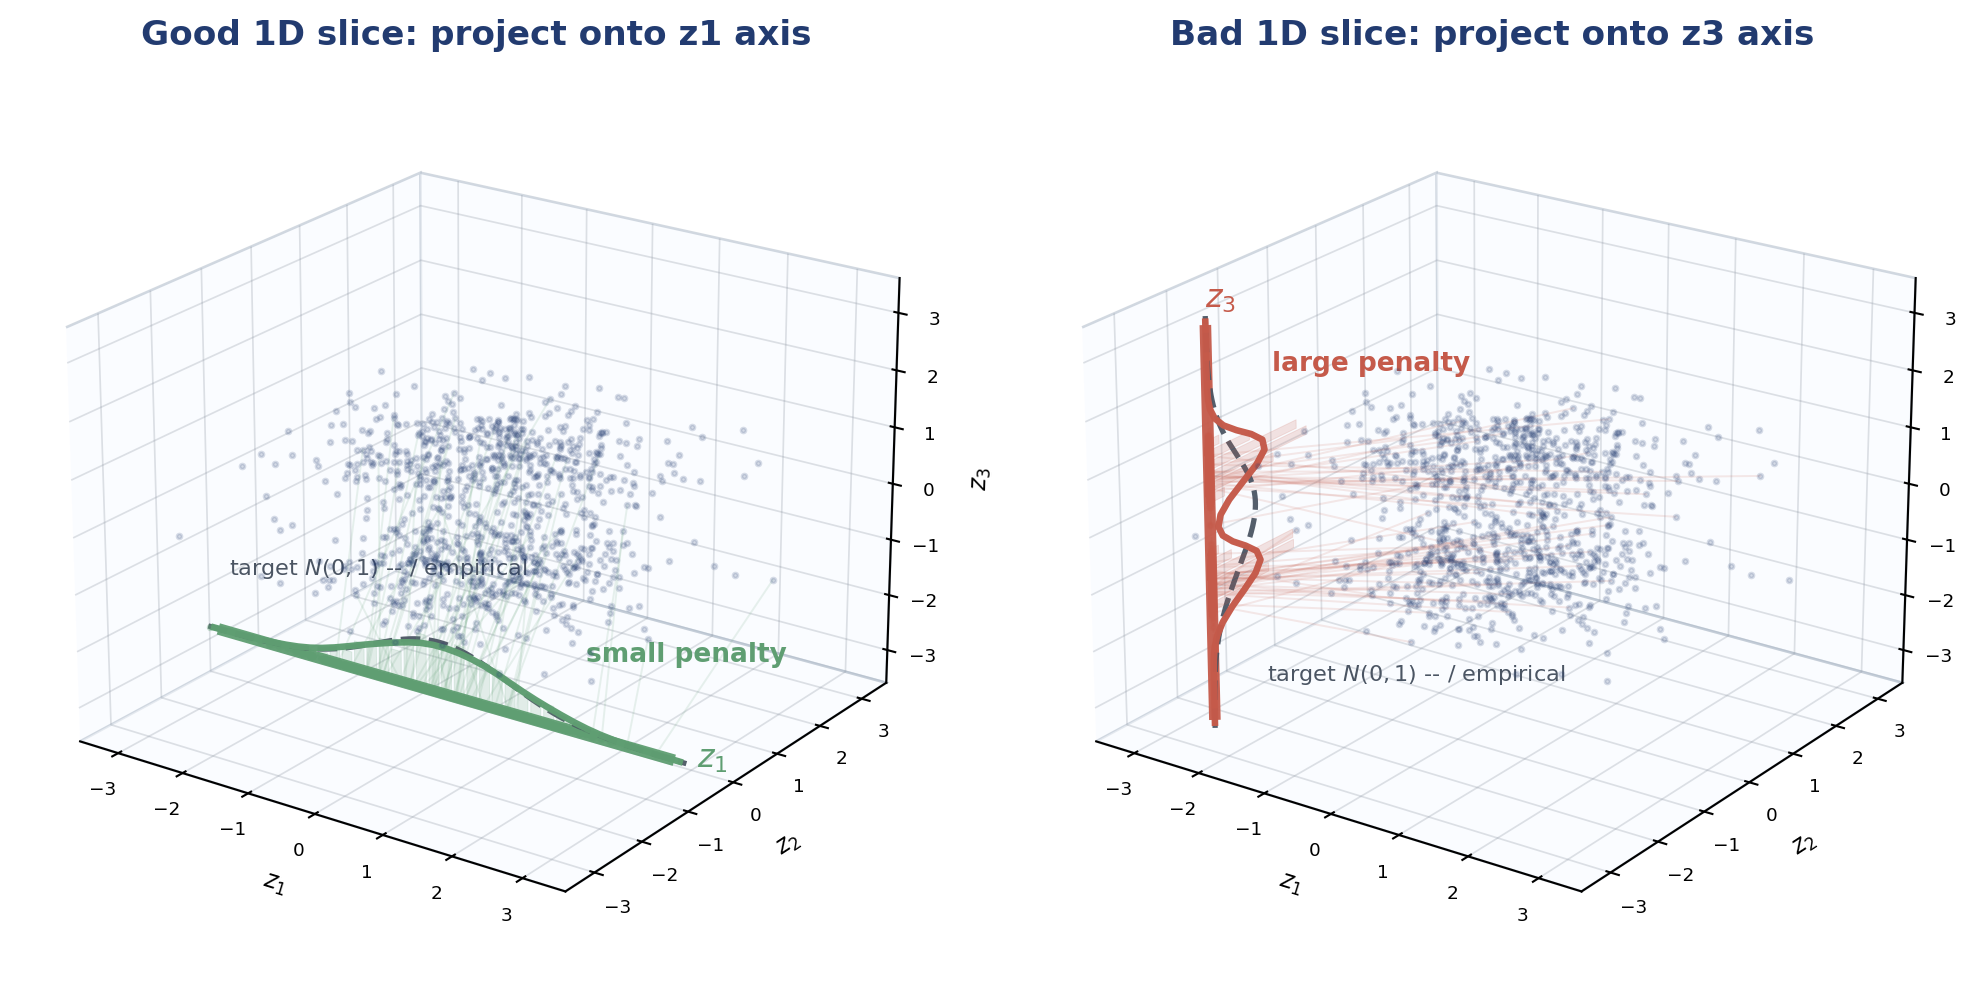
\includegraphics[width=\textwidth,height=0.71\textheight,keepaspectratio]{sigreg_bad_projection_lines.png}
\end{center}

\vspace{-0.7em}
{\tiny\color{mgray}
\textbf{Ghi chú:} Hình tạo bằng matplotlib từ dữ liệu mô phỏng ($z_1,z_2\sim\mathcal{N}(0,1)$, $z_3$ không chuẩn) để trực quan hóa các slice 1D; không phải kết quả thực nghiệm.
}

\vspace{0.15em}
\begin{mdframed}[
  linecolor=maccent, linewidth=1.5pt,
  backgroundcolor=mlightgold,
  innertopmargin=5pt, innerbottommargin=5pt,
  innerleftmargin=10pt, innerrightmargin=10pt,
  roundcorner=3pt, skipabove=2pt, skipbelow=0pt
]
\centering\small\bfseries\color{mprimary}
Trong ví dụ này, slice $z_1$ và $z_2$ gần chuẩn nên penalty nhỏ.\\[-1pt]
Slice $z_3$ lệch khỏi đường chuông chuẩn nên test 1D cho score lớn và SIGReg phạt.
\end{mdframed}
\end{frame}


% ─── [MERGED] SIGReg: trực giác + định nghĩa (code đã bỏ) ────────────────────
\begin{frame}{SIGReg: Từ Trực Giác Đến Định Nghĩa}

\vfill
% 1) Trực giác (trên, nhỏ)
\begin{center}
\textbf{Trực giác (Cramér–Wold):} hai phân phối bằng nhau $\iff$ mọi hình chiếu 1D bằng nhau.\\[3pt]
$X \stackrel{d}{=} Y \iff
  \langle \mathbf{u}, X\rangle \stackrel{d}{=}
  \langle \mathbf{u}, Y\rangle,\;\forall \mathbf{u}\in\mathbb{S}^{K-1}$
\end{center}

\vspace{0.6em}

% 2) Định nghĩa — hero card bo góc, căn giữa
\begin{center}
\begin{mdframed}[roundcorner=9pt, linewidth=1.2pt, linecolor=mprimary!55,
    backgroundcolor=mlight, userdefinedwidth=0.76\textwidth, align=center,
    innertopmargin=9pt, innerbottommargin=9pt, innerleftmargin=14pt, innerrightmargin=14pt]
\centering
{\color{mprimary}\textbf{Định nghĩa — SIGReg}}\\[7pt]
$\displaystyle
  \mathrm{SIGReg}_T(\mathbb{A},\{f_\theta(\mathbf{x}_n)\})
  \triangleq \frac{1}{|\mathbb{A}|}\sum_{\mathbf{a}\in\mathbb{A}}
  T\!\left(\{\mathbf{a}^\top f_\theta(\mathbf{x}_n)\}\right)$\\[7pt]
{\footnotesize\color{mgray} $\mathbb{A}$: $M$ hướng trên $\mathbb{S}^{K-1}$ $\cdot$ $T$ = Epps-Pulley $\cdot$ average}
\end{mdframed}
\end{center}

\vspace{0.9em}
% 3) Ba tính chất — chip keyword bo góc
\begin{center}
\begin{tikzpicture}[
    chip/.style={draw=mgood!45, fill=mlightsage, rounded corners=8pt,
                 minimum width=3.5cm, minimum height=1.45cm, align=center, inner sep=6pt}]
  \node[chip] (c1) at (0,0)    {\footnotesize\textbf{\color{mgood!55!black}Ý nghĩa}\\[4pt] embedding $\to \mathcal{N}(0,I)$};
  \node[chip] (c2) at (4.15,0) {\footnotesize\textbf{\color{mgood!55!black}Ổn định}\\[4pt] $\nabla$ chặn bởi $4\sigma^2/N$};
  \node[chip] (c3) at (8.3,0)  {\footnotesize\textbf{\color{mgood!55!black}Rẻ}\\[4pt] $\mathcal{O}(N)\,\cdot\,$DDP-friendly};
\end{tikzpicture}
\end{center}
\vfill

\end{frame}


% ─── Slide 8: LeJEPA loss ─────────────────────────────────────────────────────
\begin{frame}{LeJEPA: Một Công Thức, Một Siêu Tham Số}

\begin{center}
\[
  \mathcal{L}_{\rm LeJEPA}
  = \underbrace{(1-\lambda)\cdot\mathcal{L}_{\rm pred}}_{\displaystyle\text{views phải agree}}
  \;+\;
  \underbrace{\lambda\cdot\text{SIGReg}}_{\displaystyle\text{push về }\mathcal{N}(\mathbf{0},I)}
\]
\end{center}

\vspace{-0.3em}
\begin{center}
\resizebox{0.72\linewidth}{!}{
\begin{tikzpicture}[
    every node/.style={font=\small},
    viewbox/.style={pbox, minimum width=1.6cm, minimum height=0.6cm, font=\scriptsize, align=center},
    encbox/.style={darkbox, minimum width=1.6cm, minimum height=3.6cm, align=center},
    projbox/.style={pbox, fill=mprimary!10, draw=mprimary, minimum width=1.6cm, minimum height=2.6cm, align=center},
    lossbox/.style={rectangle, draw, rounded corners=3pt, thick, align=center, minimum height=0.7cm, font=\scriptsize, inner sep=4pt}
  ]
  
  % Inputs
  \node[font=\small\bfseries, draw=mgray, rounded corners, inner sep=4pt, text=mprimary] (img) at (0, 0) {Image $\mathbf{x}$};
  
  % Views
  \node[viewbox] (v1) at (3, 1.8) {view 1\\(global)};
  \node[viewbox] (v2) at (3, 0.6) {view 2\\(global)};
  \node[font=\small, mgray] (vd) at (3, -0.4) {$\vdots$};
  \node[viewbox] (v8) at (3, -1.4) {view 8\\(local)};
  
  \draw[->, thick, mgray] (img) |- (v1) node[pos=0.75, above=0pt, font=\tiny] {aug};
  \draw[->, thick, mgray] (img) |- (v2) node[pos=0.75, above=0pt, font=\tiny] {aug};
  \draw[->, thick, mgray] (img) |- (v8) node[pos=0.75, above=0pt, font=\tiny] {aug};
  
  % Encoder
  \node[encbox] (enc) at (5.8, 0.2) {Encoder\\$f_\theta$\\ \tiny(bất kỳ)};
  \draw[->, thick, mgray] (v1) -- (v1 -| enc.west);
  \draw[->, thick, mgray] (v2) -- (v2 -| enc.west);
  \draw[->, thick, mgray] (v8) -- (v8 -| enc.west);
  
  % Projector
  \node[projbox] (proj) at (8.3, 0.2) {Proj Head\\ \tiny(3-layer MLP)};
  \draw[->, thick, mgray] (enc) -- (proj);
  
  % z
  \node[circle, draw=mprimary, thick, fill=white, inner sep=1.5pt, font=\normalsize\bfseries, text=mprimary] (z) at (10.6, 0.2) {$\mathbf{z}$};
  \draw[->, thick, mprimary] (proj) -- (z);
  
  % Losses
  \node[lossbox, draw=mbad, fill=mbad!10, text=mbad!80!black] (inv) at (7.4, -2.4) {\textbf{Invariance Loss}\\$\mathcal{L}_{\rm pred} \; (\mathbf{z}_v \approx \boldsymbol{\mu})$};
  \node[lossbox, draw=mgood, fill=mgood!10, text=mgood!80!black] (sig) at (10.6, -2.4) {\textbf{SIGReg Loss}\\$\mathbf{z} \sim \mathcal{N}(0, I)$};
  
  \draw[->, mbad, thick, rounded corners] (z.south) |- (8.8, -1.4) -| (inv.north);
  \draw[->, mgood, thick] (z.south) -- (sig.north);
  
\end{tikzpicture}
}
\end{center}

\takeaway{1 loss · 1 hyperparameter · 0 heuristic · lý thuyết từ first principles}

\end{frame}


% ─── [BATCH 3] Curse of dimensionality ───────────────────────────────────────
% \begin{frame}{SIGReg Vượt Qua Curse of Dimensionality}

% \begin{columns}[T]
% \column{0.50\textwidth}

% \textbf{Định lý 5 (Unified Error Bound):}\\[4pt]
% Khoảng cách thực sự giữa không gian Latent và $\mathcal{N}(0,I)$ luôn bị chặn trên bởi $\mathcal{O}\big(M^{-\frac{2\alpha}{K-1}}\big)$, với $\alpha$ là độ trơn (smoothness) của dữ liệu.

% \vspace{0.6em}
% \begin{tikzpicture}
% \begin{axis}[
%   width=5.2cm, height=3.2cm,
%   xlabel={$M$ (số hướng, log-scale)}, ylabel={Sai số kỳ vọng},
%   xmode=log,
%   xlabel style={font=\small}, ylabel style={font=\small},
%   tick label style={font=\tiny},
%   xmin=16, xmax=2048, ymin=0, ymax=1200,
%   grid=major, grid style={mgray!15},
%   legend pos=outer north east,
%   legend style={font=\tiny, draw=none, fill=mgray!5, inner sep=2pt, nodes={inner sep=1pt}},
% ]
%   \addplot[mbad, thick, domain=16:2048, samples=30]
%     {1100*exp(-x/800)};
%   \addlegendentry{Fixed $\mathbb{A}$}
%   \addplot[mgood, very thick, domain=16:2048, samples=30]
%     {1100*exp(-x/120)};
%   \addlegendentry{Resampled (SGD)}
% \end{axis}
% \end{tikzpicture}

% \column{0.46\textwidth}
% \vspace{0.3em}

% \textbf{Hai lý do SIGReg thắng curse:}

% \vspace{0.4em}
% \begin{primarybox}
% \footnotesize \textbf{1. Sobolev smoothness $\alpha$:} DNN tự nhiên smooth (BatchNorm, Dropout, weight decay) $\Rightarrow$ $\alpha$ lớn $\Rightarrow$ tốc độ hội tụ $|\mathbb{A}|^{-2\alpha/(K-1)}$ nhanh $\Rightarrow$ $M=\mathcal{O}(K)$ là đủ.
% \end{primarybox}

% \vspace{0.4em}
% \begin{primarybox}
% \footnotesize \textbf{2. SGD resampling:} Mỗi mini-batch lấy mẫu lại $M$ hướng mới $\Rightarrow$ sau $T$ bước huấn luyện, số hướng tích lũy $=M\times T$ $\Rightarrow$ coverage tăng miễn phí.
% \end{primarybox}

% \vspace{0.4em}
% \begin{goodbox}
% \footnotesize $M=16$ hướng mỗi bước đủ để match $K=2048$-dim embedding, nhờ resampling compounding.
% \end{goodbox}

% \end{columns}
% \end{frame}


% ─── [BATCH 3] Lambda tradeoff ────────────────────────────────────────────────
% Comment lại theo yêu cầu — giữ nội dung, không xóa.
\iffalse
\begin{frame}{$\lambda$: Nút Điều Chỉnh Duy Nhất}

\begin{columns}[T]
\column{0.50\textwidth}

\begin{tikzpicture}[every node/.style={font=\small}, scale=0.9]
  % Spectrum
  \draw[->, thick, mgray!60] (0,0) -- (6.5,0) node[right,font=\tiny]{$\lambda$};

  % lambda=0
  \draw[thick,mgray] (0.3,0.15)--(0.3,-0.15);
  \node[font=\tiny,below=2pt] at (0.3,0) {$0$};
  \node[mbad, font=\tiny, align=center] at (0.3, 1.1)
    {Pure Pred.\\Collapse};
  \fill[mbad!20] (0.3,0.45) circle (0.25cm);
  \fill[mbad] (0.3,0.45) circle (0.05cm);

  % lambda=1
  \draw[thick,mgray] (6.2,0.15)--(6.2,-0.15);
  \node[font=\tiny,below=2pt] at (6.2,0) {$1$};
  \node[mbad, font=\tiny, align=center] at (6.2, 1.1)
    {Pure SIGReg\\Uniform};
  \foreach \px/\py in {5.95/0.5, 6.25/0.35, 6.0/0.3, 6.3/0.55, 6.15/0.45}{
    \fill[mbad!60] (\px,\py) circle (0.04cm);
  }

  % sweet spot
  \draw[thick, mgood, line width=1.5pt] (2.2,0.15)--(2.2,-0.15);
  \node[font=\tiny,below=2pt,mgood] at (2.2,0) {$0.05$};
  \node[mgood, font=\small\bfseries, align=center] at (2.2, 1.2)
    {Sweet spot};
  \fill[mgood!20] (2.2,0.5) circle (0.32cm);
  \foreach \px/\py in {2.05/0.6, 2.35/0.42, 2.0/0.42, 2.38/0.6, 2.2/0.5}{
    \fill[mgood!70] (\px,\py) circle (0.04cm);
  }

  % brace
  \draw[decorate, decoration={brace, amplitude=4pt}, mgood!70, thick]
    (3.2,-0.45) -- (1.3,-0.45)
    node[midway,below=4pt,font=\tiny,mgood]{vùng ổn định};
\end{tikzpicture}

\vspace{0.3em}
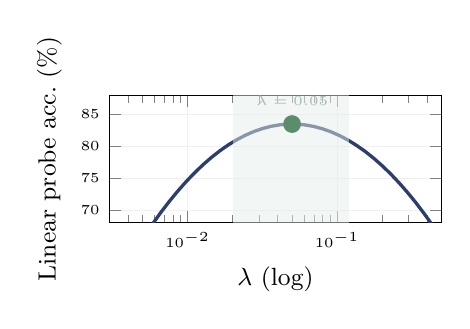
\begin{tikzpicture}
\begin{axis}[
  width=5.8cm, height=3.2cm,
  xlabel={$\lambda$ (log)}, ylabel={Linear probe acc.\ (\%)},
  xmode=log, xlabel style={font=\small}, ylabel style={font=\small},
  tick label style={font=\tiny},
  xmin=0.003, xmax=0.5, ymin=68, ymax=88,
  grid=major, grid style={mgray!15},
]
  \addplot[mprimary, very thick, domain=0.003:0.5, samples=40]
    {83.5 - 18*(log10(x) - log10(0.05))^2};
  \addplot[mark=*, mgood, mark size=3pt] coordinates {(0.05,83.5)}
    node[above=3pt,font=\tiny,mgood]{$\lambda=0.05$};
  \fill[mgood!15,opacity=0.5] (axis cs:0.02,68) rectangle (axis cs:0.12,88);
\end{axis}
\end{tikzpicture}

\column{0.46\textwidth}
\vspace{0.3em}

\begin{primarybox}
\footnotesize \textbf{Config mặc định:} $\lambda=0.05 \cdot V=2g+6l \cdot bs \geq 128 \cdot M=1024 \cdot 17\text{ pts, } t\in[-5,5]$.
\end{primarybox}

\vspace{1.5em}
\begin{goodbox}
\footnotesize \textbf{Robust:} $\lambda \in [0.01, 0.1]$ (Fig.8).
\end{goodbox}

\end{columns}
\end{frame}
\fi % ─── hết bản comment "λ: Nút Điều Chỉnh Duy Nhất" ────────────────────────


% ─── [BATCH 3] LeJEPA vs prior + VICReg relation ─────────────────────────────
% Comment lại theo yêu cầu — giữ nội dung, không xóa.
\iffalse
\begin{frame}{LeJEPA Generalizes VICReg — Và Giải Thích Tại Sao VICReg Bị Hạn Chế}

\begin{columns}[T]
\column{0.48\textwidth}

\textbf{Sự kết nối lý thuyết:}\\[4pt]
Nếu thay thế hàm Test $T$ trong SIGReg bằng \textbf{hàm tính Moment} (chỉ đo trung bình và phương sai), SIGReg sẽ hội tụ chính xác về \textbf{VICReg}.

\vspace{0.8em}
\begin{tikzpicture}[every node/.style={font=\footnotesize}, scale=0.95]
  \node[darkbox, minimum width=3.4cm, minimum height=0.65cm, align=center]
    (lj) at (0,0) {\textbf{LeJEPA}\\(Framework Tổng Quát)};

  \node[gbox, minimum width=3.4cm, minimum height=0.65cm, align=center]
    (ep) at (0,-1.4) {$T$ = \textbf{Epps-Pulley}\\(Khuyên dùng: Toàn diện)};

  \node[pbox, minimum width=3.4cm, minimum height=0.65cm, align=center]
    (vc) at (0,-2.8) {$T$ = \textbf{Moments}\\$\Rightarrow$ Trở thành \textbf{VICReg}};

  \node[rbox, minimum width=3.4cm, minimum height=0.65cm, align=center]
    (jb) at (0,-4.2) {$T$ = \textbf{Jarque-Bera}\\(Không ổn định)};

  \draw[arr, mgray] (lj)--(ep); 
  \draw[darr, mgray] (lj.west) to[out=180,in=180] node[left=1pt, font=\tiny, align=right]{case\\đặc biệt} (vc.west);
  \draw[darr, mgray] (lj.west) to[out=180,in=180] node[left=1pt, font=\tiny, align=right]{case\\đặc biệt} (jb.west);
\end{tikzpicture}

\column{0.48\textwidth}
\vspace{0.3em}

\textbf{Tại sao VICReg không đủ?}

\vspace{0.3em}
\begin{badbox}
\footnotesize \textbf{Định lý 3:} VICReg chỉ đối chiếu 2 moment đầu ($\hat\mu, \hat\sigma^2$) $\Rightarrow$ Dễ dính \textbf{shortcut} (nhiều phân phối khác nhau có cùng $\hat\mu, \hat\sigma^2$).\\[2pt]
$\Rightarrow$ Phải chắp vá bằng các heuristic phụ để tránh sụp đổ.
\end{badbox}

\vspace{0.6em}
\begin{goodbox}
\footnotesize \textbf{SIGReg:} Ràng buộc \textbf{toàn bộ} đặc trưng phân phối qua ECF $\Rightarrow$ Đảm bảo hội tụ tuyệt đối (Cramér-Wold).
\end{goodbox}

\vspace{0.6em}
\begin{accentbox}
\footnotesize \textbf{Kết luận:} VICReg thực chất là một phiên bản giới hạn và thiếu chặt chẽ của LeJEPA.
\end{accentbox}

\end{columns}
\end{frame}
\fi % ─── hết bản comment "LeJEPA Generalizes VICReg" ────────────────────────


% ─── SECTION DIVIDER ──────────────────────────────────────────────────────────
\section{Kết quả}


% % ─── Slide 9: Training loss + in-domain ──────────────────────────────────────
% \begin{frame}{Hai Kết Quả Nổi Bật}

% \begin{columns}[T]
% \column{0.48\textwidth}

% \textbf{Loss huấn luyện dự báo downstream performance}

% \vspace{0.2em}
% \begin{tikzpicture}
% \begin{axis}[
%   width=5.8cm, height=4.0cm,
%   xlabel={Test acc.\ (\%)},
%   ylabel={Loss huấn luyện},
%   ymode=log,
%   xlabel style={font=\small},
%   ylabel style={font=\small},
%   tick label style={font=\tiny},
%   xmin=0, xmax=72,
%   ymin=0.4, ymax=12,
%   grid=major, grid style={mgray!15},
% ]
%   % Simulated scatter (trend from paper)
%   \addplot[only marks, mark=*, mark size=1.6pt,
%            mprimary!60, opacity=0.75]
%     coordinates {
%       (5,9.5)(10,7.2)(15,5.5)(18,4.2)(22,3.4)
%       (27,2.6)(32,2.1)(38,1.7)(44,1.4)(50,1.1)
%       (56,0.9)(62,0.75)(68,0.62)(8,8.5)(14,6.0)
%       (20,4.8)(25,3.0)(35,2.3)(42,1.85)(55,1.0)
%     };
%   \addplot[maccent, very thick, domain=3:70, samples=30]
%     {7.5*exp(-x/14)};
%   \node[font=\tiny, maccent, fill=white, inner sep=1pt]
%     at (axis cs:50, 2.8) {$\rho_s \approx 94\%$ Spearman};
% \end{axis}
% \end{tikzpicture}

% \column{0.48\textwidth}

% \textbf{In-domain SSL đánh bại frontier models}\\
% \footnotesize Galaxy10 (11K ảnh thiên hà):

% \vspace{0.2em}
% \begin{tikzpicture}
% \begin{axis}[
%   width=5.2cm, height=4.0cm,
%   xlabel={Số mẫu mỗi lớp},
%   ylabel={Accuracy (\%)},
%   xmode=log,
%   xlabel style={font=\small},
%   ylabel style={font=\small},
%   tick label style={font=\tiny},
%   xmin=0.8, xmax=250,
%   ymin=15, ymax=88,
%   grid=major, grid style={mgray!15},
%   legend pos=outer north east,
%   legend style={font=\tiny, draw=none, fill=mgray!5, inner sep=2pt, nodes={inner sep=1pt}},
% ]
%   \addplot[mgray!70, thick, mark=square*, mark size=1.5pt]
%     coordinates {(1,21)(2,22)(5,30)(10,36)(100,61)(180,68)};
%   \addlegendentry{DINOv2}
%   \addplot[mgray!50, thick, mark=triangle*, mark size=1.5pt, dashed]
%     coordinates {(1,25)(2,29)(5,37)(10,45)(100,70)(180,73)};
%   \addlegendentry{DINOv3}
%   \addplot[mgood, very thick, mark=*, mark size=2pt]
%     coordinates {(1,31)(2,38)(5,52)(10,61)(100,75)(180,78)};
%   \addlegendentry{LeJEPA}
% \end{axis}
% \end{tikzpicture}
% \end{columns}

% \vspace{0.4em}
% \begin{columns}[T]
% \column{0.48\textwidth}
% \begin{primarybox}
% \footnotesize Lần đầu trong SSL: loss huấn luyện \textbf{tương quan 94\%} với accuracy — chọn model không cần linear probe.
% \end{primarybox}

% \column{0.48\textwidth}
% \begin{goodbox}
% \footnotesize Domain-specific SSL $>$ frontier transfer — ngay cả khi chỉ có 11K samples.
% \end{goodbox}
% \end{columns}

% \end{frame}


% % ─── Slide 10: Scale ─────────────────────────────────────────────────────────
% \begin{frame}{Scale: 60+ Kiến Trúc, Không Collapse, SOTA}

% \begin{columns}[T]
% \column{0.46\textwidth}
% \vspace{0.2em}

% 50 models, 8 architecture families, ImageNet-10:

% \begin{tikzpicture}
% \begin{axis}[
%   width=5.6cm, height=4.2cm,
%   xlabel={Parameters (M)},
%   ylabel={Top-1 Acc.\ (\%)},
%   xlabel style={font=\small},
%   ylabel style={font=\small},
%   tick label style={font=\tiny},
%   xmin=1, xmax=20, ymin=90, ymax=96,
%   grid=major, grid style={mgray!15},
%   legend style={font=\tiny, at={(1.05,0.5)},
%                 anchor=west, draw=none},
% ]
%   \addplot[only marks, mark=*, mark size=2pt, mprimary!80]
%     coordinates {(6,92.5)(10,93.2)(14,93.8)(17,94.1)(19,94.5)};
%   \addlegendentry{ResNet}
%   \addplot[only marks, mark=square*, mark size=2pt, mgood]
%     coordinates {(5,92.9)(9,94.0)(13,94.6)(16,95.0)};
%   \addlegendentry{ViT}
%   \addplot[only marks, mark=triangle*, mark size=2pt, maccent!90]
%     coordinates {(3,91.5)(7,92.2)(11,92.8)(18,93.5)};
%   \addlegendentry{Khác}
%   \draw[<->, mbad, thick] (axis cs:1.2,91.5) -- (axis cs:1.2,95.0)
%     node[midway, left=1pt, font=\tiny, mbad]{3.5\%};
% \end{axis}
% \end{tikzpicture}

% \textcolor{mgood}{\textbf{Không collapse nào}} trong tất cả 50 models.

% \column{0.50\textwidth}
% \vspace{0.3em}

% \begin{accentbox}
% \footnotesize\bfseries ImageNet-1K · ViT-H/14 · 100 epochs:
% \begin{center}
% {\Huge\bfseries\color{mprimary} 79.0\%}\\[3pt]
% \small linear probe, frozen backbone
% \end{center}
% \end{accentbox}

% \vspace{0.4em}
% \begin{tabular}{@{}lrr@{}}
% \toprule
% Method & Params & Acc \\
% \midrule
% I-JEPA ViT-H (300ep) & 632M & 77.3\% \\
% LeJEPA ViT-L (100ep) & 304M & 78.2\% \\
% \textbf{LeJEPA ConvNeXt-H} & 660M & \textbf{79.0\%} \\
% \bottomrule
% \end{tabular}

% \vspace{0.4em}
% \begin{goodbox}
% \footnotesize 3$\times$ ít compute · model nhỏ hơn · vẫn SOTA.
% \end{goodbox}

% \end{columns}

% \end{frame}


% % ─── [BATCH 4] Ablation stability ────────────────────────────────────────────
% \begin{frame}{Ablation: LeJEPA Ổn Định Trên Mọi Siêu Tham Số}

% \begin{columns}[T]
% \column{0.50\textwidth}

% \textbf{Epps-Pulley hyperparameters} (ViT-L/14, ImageNet-1K, 100ep):

% \vspace{0.3em}
% \begin{tabular}{@{}ccrrrr@{}}
% \toprule
% Integ. & $M$ & \multicolumn{3}{c}{\# quad. points} \\
% \cmidrule(lr){3-5}
%  & & 5 & 17 & 41 \\
% \midrule
% $[-1,1]$ & 512  & 71.8 & 72.1 & 72.0 \\
% $[-3,3]$ & 512  & 74.0 & 74.2 & 74.0 \\
% $[-5,5]$ & 512  & 73.7 & \textbf{74.2} & 74.2 \\
% $[-5,5]$ & 2048 & 74.5 & \textbf{74.8} & 74.8 \\
% \bottomrule
% \end{tabular}

% \vspace{0.5em}
% \textbf{Register tokens:} không cần thiết.

% \vspace{0.2em}
% \begin{tabular}{@{}lrr@{}}
% \toprule
% reg\_tokens & $M=1024$ & $M=4096$ \\
% \midrule
% 0 & 75.14 & 75.61 \\
% 2 & 75.08 & 75.67 \\
% 8 & 75.23 & 75.84 \\
% \bottomrule
% \end{tabular}

% \column{0.46\textwidth}
% \vspace{0.3em}

% \textbf{So sánh vs DINO/I-JEPA:}

% \vspace{0.3em}
% \begin{tabular}{@{} >{\footnotesize}l >{\footnotesize\color{mbad}}c >{\footnotesize\color{mbad}}c >{\footnotesize\color{mgood}\bfseries}c @{}}
% \toprule
% \footnotesize Tiêu chí & \footnotesize DINO & \footnotesize I-JEPA & \footnotesize LeJEPA \\
% \midrule
% Anti-collapse   & EMA+sg  & sg+mask & Theorem \\
% \# Hyperparams  & $\geq$7 & $\geq$5 & 1 ($\lambda$) \\
% Complexity      & $\mathcal{O}(N)$ & $\mathcal{O}(N)$ & $\mathcal{O}(N)$ \\
% Architecture    & ViT     & ViT     & Any (60+) \\
% Loss corr.      & ${\sim}20\%$ & ${\sim}30\%$ & 94\% \\
% Core code       & 1000+   & 500+    & $\approx$50 \\
% \bottomrule
% \end{tabular}

% \vspace{0.5em}
% \begin{accentbox}
% \footnotesize Không có collapse nào trong tất cả 50+ models, không tinh chỉnh siêu tham số theo kiến trúc.
% \end{accentbox}

% \end{columns}
% \end{frame}


% ─── Reproduce: ViT-B/16 5 epoch trên IN-1K ──────────────────────────────────
\begin{frame}{Reproduce — LeJEPA ViT-B/16, 5 epoch pretrain trên ImageNet-1K}

% Bối cảnh — 1 dòng, căn giữa
\begin{center}
{\footnotesize\color{mgray}\textbf{Setup:} \kw{ViT-B/16} \emph{from scratch}, IN-1K, \textbf{5 epoch}, $\lambda=0.05$, 1024 slices, 2+4 views, AdamW/bf16.}
\end{center}

\vspace{0.5em}
\begin{center}
\small
\textbf{Linear probe} — top1 (\%), frozen backbone, 8 dataset transfer (few-shot 1/10 trung bình 3 seed; \emph{all} = full train, 1 lần):\\[0.5em]
\renewcommand{\arraystretch}{1.25}
\begin{tabular}{@{}l rrrrrrrr >{\columncolor{mlight}\bfseries}r@{}}
\toprule
shots & DTD & Aircraft & Cars & CIFAR-10 & CIFAR-100 & Flowers & Food & Pets & avg. \\
\midrule
1   & 18.4 &  4.0 &  2.4 & 26.5 & 10.8 & 31.0 &  6.1 & 11.8 & 13.9 \\
10  & 40.6 & 11.0 &  9.0 & 52.3 & 32.3 & 68.5 & 22.3 & 30.7 & 33.3 \\
all & 58.2 & 26.0 & 19.5 & 82.8 & 63.3 & 83.2 & 56.9 & 50.0 & 55.0 \\
\bottomrule
\end{tabular}
\end{center}

\vspace{0.4em}
\begin{center}
{\footnotesize\color{mgray}\textbf{\color{mgood!60!black}Đọc:} coarse (Flowers, CIFAR) học sớm; fine-grained (Aircraft, Cars) cần pretrain dài hơn.}
\end{center}

\takeaway{5 epoch scratch trên IN-1K $\Rightarrow$ 55\% avg linear probe — pipeline ổn định đúng như paper.}

\end{frame}


% ─── Ablation A: siêu tham số của mục tiêu học ───────────────────────────────
\begin{frame}{Ablation A — Siêu tham số của mục tiêu học (SIGReg \& multi-view)}

{\small\textbf{\color{mbad}Câu hỏi:} SIGReg nhạy thế nào với lưới tích phân Epps-Pulley? Cần bao nhiêu view (tổng / global)?}
\vspace{0.4em}

\begin{columns}[T]
\column{0.52\textwidth}
\scriptsize
\hspace*{0.8cm}\textbf{Epps-Pulley} — top1 (\%), đủ 27 cấu hình:\\[0.2em]
\hspace*{0.8cm}\begin{tabular}{@{}llccc@{}}
\toprule
integ. & slices & \multicolumn{3}{c}{\texttt{n\_points}} \\
\cmidrule(lr){3-5}
 & & 5 & 17 & 41 \\
\midrule
$[-1,1]$ & 512  & 59.3 & 59.5 & 60.6 \\
         & 1024 & 63.8 & 63.9 & 63.2 \\
         & 4096 & \textbf{70.1} & 69.5 & 69.2 \\
$[-3,3]$ & 512  & 55.6 & 55.4 & 56.1 \\
         & 1024 & 60.8 & 59.5 & 60.0 \\
         & 4096 & 67.1 & 67.3 & 67.0 \\
$[-5,5]$ & 512  & 57.6 & 54.9 & 55.1 \\
         & 1024 & 58.2 & 59.2 & 59.2 \\
         & 4096 & 63.3 & 66.8 & 66.8 \\
\bottomrule
\end{tabular}

\vspace{0.4em}
\hspace*{0.8cm}\textbf{Số view} ($V$): \; 4:\,\textbf{72.8} \; 6:\,65.7 \; 8:\,60.6 \; 10:\,57.1

\column{0.46\textwidth}
\centering

\includegraphics[width=\linewidth]{A_epps_heatmap.pdf}\\[0.4em]

\includegraphics[width=0.60\linewidth]{B_views_heatmap.pdf}
\end{columns}

\takeaway{Chỉ \texttt{num\_slices} là đòn bẩy thật; \texttt{n\_points}/$t_{\max}$ gần như trung tính.}

\end{frame}


% ─── Ablation B: thành phần kiến trúc ────────────────────────────────────────
\begin{frame}{Ablation B — Thành phần kiến trúc (nơi \& cách áp mục tiêu)}

{\small\textbf{\color{mbad}Câu hỏi:} Áp SIGReg ở đâu (proj/embed)? Projector cần phi tuyến? Có cần predictor? Token nào nuôi projector?}

{\centering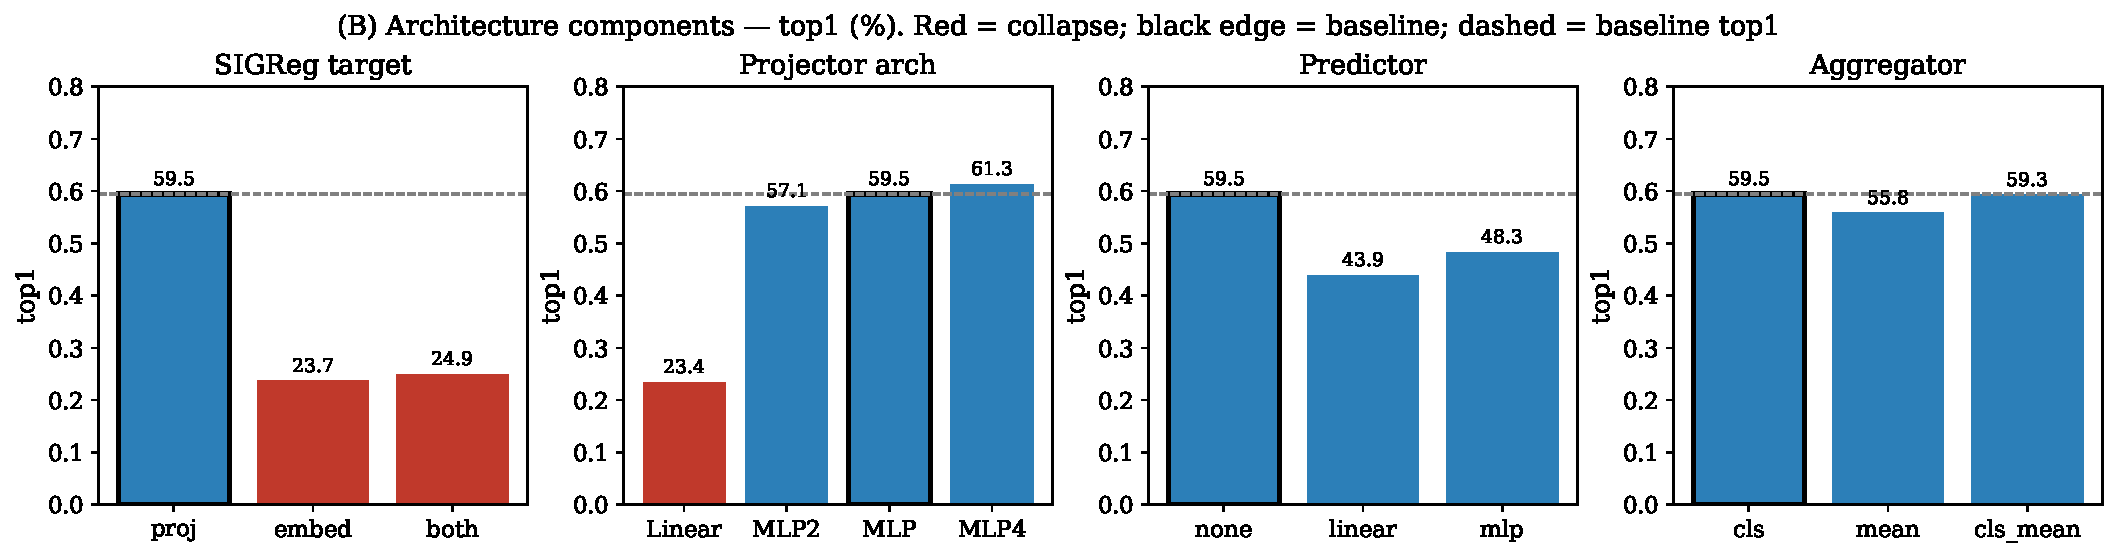
\includegraphics[width=0.80\linewidth]{E_arch_bars.pdf}\par}

\begin{columns}[T]
\column{0.56\textwidth}
\scriptsize
\begin{tabular}{@{}ll@{}}
\toprule
Thành phần & top1 (tốt $\to$ tệ) \\
\midrule
SIGReg target & proj \textbf{59.5} $\gg$ \textcolor{mbad}{embed 23.7 / both 24.9} \\
Projector     & MLP4 61.3 $>$ MLP 59.5 $>$ MLP2 $>$ \textcolor{mbad}{Linear 23.4} \\
Predictor     & \textbf{none 59.5} $\gg$ mlp 48.3 $>$ linear 43.9 \\
Aggregator    & cls \textbf{59.5} $\approx$ cls\_mean $>$ mean 55.8 \\
\bottomrule
\end{tabular}

\column{0.44\textwidth}
\footnotesize
\textbf{\color{mgood}Trả lời:}
\begin{itemize}\itemsep1pt
  \item SIGReg \textbf{bắt buộc} trên projection; projector \textbf{phải phi tuyến} — đặt sai $\Rightarrow$ collapse
  \item \textbf{Không cần predictor}; CLS đơn đã đủ
\end{itemize}
\end{columns}

\takeaway{Đặt SIGReg đúng chỗ + projector phi tuyến $\Rightarrow$ tự chống collapse, khỏi cần predictor.}

\end{frame}


% ─── Ablation C: regularization augmentation ─────────────────────────────────
\begin{frame}{Ablation C — Regularization kiểu augmentation}

{\small\textbf{\color{mbad}Câu hỏi:} Tỉ lệ patch-masking nào tối ưu? LeJEPA nhạy với stochastic depth (drop-path) không?}
\vspace{0.4em}

\begin{columns}[T]
\column{0.54\textwidth}
\centering
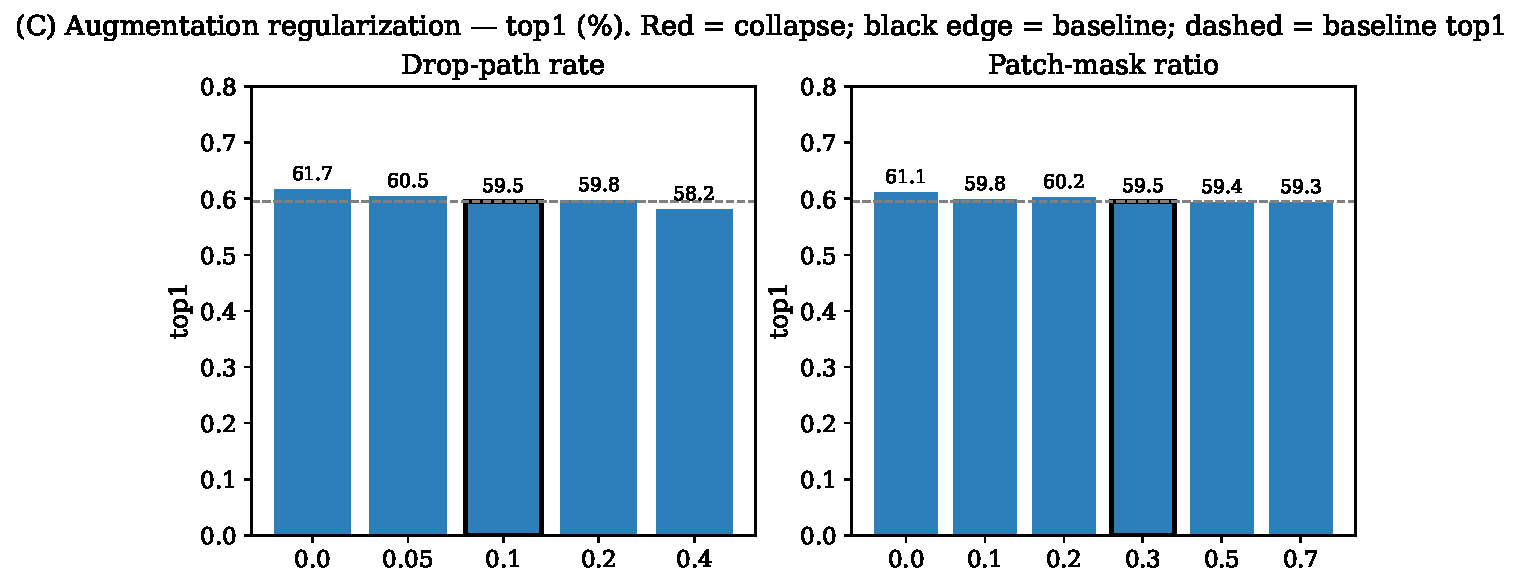
\includegraphics[width=\linewidth]{F_reg_bars.pdf}

\column{0.44\textwidth}
\scriptsize
\textbf{Patch-mask ratio:}\\[0.2em]
\begin{tabular}{@{}lcccccc@{}}
\toprule
ratio & 0.0 & 0.1 & 0.2 & 0.3 & 0.5 & 0.7 \\
\midrule
top1 & \textbf{61.1} & 59.8 & 60.2 & 59.5 & 59.4 & 59.3 \\
\bottomrule
\end{tabular}

\vspace{0.6em}
\textbf{Drop-path rate:}\\[0.2em]
\begin{tabular}{@{}lccccc@{}}
\toprule
rate & 0.0 & 0.05 & 0.1 & 0.2 & 0.4 \\
\midrule
top1 & \textbf{61.7} & 60.5 & 59.5 & 59.8 & 58.2 \\
\bottomrule
\end{tabular}

\vspace{0.7em}
\small\textbf{\color{mgood}Trả lời:} cả hai đạt đỉnh tại \textbf{0.0} — augmentation-reg \textbf{không giúp} ở low-data.
\end{columns}

\end{frame}


% ─── [BATCH 4] Emergent semantics ────────────────────────────────────────────
% Comment lại theo yêu cầu — giữ nội dung, không xóa.
\iffalse
\begin{frame}{Emergent Semantics: Không Supervision — Vẫn Học Được Cấu Trúc}

\begin{columns}[T]
\column{0.48\textwidth}

\textbf{PCA last-layer features} (ViT-L, ImageNet):

\vspace{0.6em}
\begin{tikzpicture}[every node/.style={font=\small}]
  %% Image placeholder (dog on grass)
  \node[inner sep=0pt, draw=mgray!40, thick, rounded corners=3pt,
        path picture={
          \node at (path picture bounding box.center) {
            
\includegraphics[width=2.4cm, height=2.4cm]{dog.png}
          };
        }] 
    (img) at (0,0) {\phantom{\rule{2.4cm}{2.4cm}}};

  %% Arrow
  \draw[->, thick, mprimary] (1.35, 0) -- (1.65, 0)
    node[above=2pt, midway, font=\tiny\bfseries]{PCA};

  %% PCA visualization — color-coded regions
  \begin{scope}[xshift=3.0cm]
    % Sky/Trees (Cool)
    \fill[cyan!15, rounded corners=3pt] (-1.2,-1.2) rectangle (1.2,1.2);
    % Grass (Cool)
    \fill[teal!25, rounded corners=3pt] (-1.2,-1.2) rectangle (1.2,-0.1);
    
    % Dog silhouette (Warm)
    \fill[maccent!80, opacity=0.9]
      plot[smooth cycle] coordinates {
        (0, 0.8)     % head top
        (0.35, 0.4)  % right ear/shoulder
        (0.45, -0.6) % right paw
        (-0.45, -0.6)% left paw
        (-0.35, 0.4) % left ear/shoulder
      };

    % Outer border
    \draw[mgray!60, thick, rounded corners=3pt] (-1.2,-1.2) rectangle (1.2,1.2);

    % Labels
    \node[font=\bfseries\tiny, white, align=center] at (0, 0.1) {dog\\(warm)};
    \node[font=\bfseries\tiny, teal!80!black, align=center] at (-0.75, 0.6) {bg\\(cool)};
    \node[font=\bfseries\tiny, teal!80!black] at (0.0,-0.85) {ground (cool)};
  \end{scope}

  \node[font=\scriptsize, mgray, align=center] at (1.5, -1.6)
    {3 PC $\to$ RGB, không dùng nhãn};
\end{tikzpicture}

\vspace{0.8em}
\textbf{Video segmentation tự động:}\\[2pt]
Thresholding attention map của CLS token giúp mask đối tượng chính xác theo frame, \emph{temporal coherence} cực mượt.

\column{0.48\textwidth}

\begin{goodbox}
\footnotesize \textbf{Warm colors} (đỏ/cam): foreground objects — chó, két, mặt.\\[5pt]
\textbf{Cool colors} (xanh lam/lục): background — cỏ, trời, lá.\\[5pt]
$\Rightarrow$ Tự động phân tách cấu trúc mà không cần bất kỳ annotation nào!
\end{goodbox}

\vspace{0.6em}
\begin{accentbox}
\footnotesize Khi tối ưu đúng chuẩn \textbf{SIGReg}, cấu trúc ngữ nghĩa (semantic structure) của dữ liệu sẽ tự nổi lên một cách tự nhiên.
\end{accentbox}

\end{columns}

\vspace{0.8em}
\begin{primarybox}
\footnotesize \textbf{Lý do cốt lõi:} Mục tiêu $\mathcal{N}(0,I)$ ép mọi hướng trong không gian embedding đều phải chứa thông tin (maximum entropy) — triệt tiêu hoàn toàn hiện tượng dimensional collapse.
\end{primarybox}
\end{frame}
\fi % ─── hết bản comment "Emergent Semantics" ────────────────────────────────

% ═══ Impact: LeWorldModel (arXiv:2603.19312) — RAG'd từ nguồn LaTeX gốc ══════
% Nguồn: arXiv-2603.19312v2/sections/{1-intro,3-method,4-exp}.tex. Tách 2 slide
% (thay vì 1 slide cũ, số liệu chung chung) vì nội dung paper giàu: cơ chế
% chuyển giao + control ở slide A; physical understanding (probing + VoE) ở
% slide B — mỗi slide có "chỗ thở" cho hero visual riêng.

% ─── Impact A: LeJEPA → LeWorldModel — cơ chế & control ──────────────────────
\begin{frame}{Tác Động Thực Tế: Từ LeJEPA Đến LeWorldModel}

% Dòng "áp dụng" — 1 dòng ngang, gọn
\begin{center}
\begin{tikzpicture}[every node/.style={font=\small}]
  \node[draw=mprimary, fill=mprimary!8, rounded corners=4pt, inner sep=5pt,
        text width=3.3cm, align=center, line width=1pt] (lejepa) at (0,0)
    {\textbf{LeJEPA}\\\scriptsize encoder tĩnh $\cdot$ SIGReg anti-collapse};
  \node[draw=mgood, fill=mgood!8, rounded corners=4pt, inner sep=5pt,
        text width=4.4cm, align=center, line width=1pt] (lewm) at (7.0,0)
    {\textbf{LeWorldModel} (arXiv:2603.19312)\\\scriptsize ViT encoder + predictor $\cdot$ dự đoán $z_{t+1}$ từ $(z_t,a_t)$};
  \draw[-{Latex[length=2.8mm]}, very thick, mprimary] (lejepa.east) -- (lewm.west)
    node[midway, above, font=\scriptsize\bfseries, mprimary]{áp dụng};
\end{tikzpicture}
\end{center}

\vspace{0.5em}
\begin{columns}[T]
\column{0.46\textwidth}

\textbf{\color{mprimary}Vẫn đúng công thức 2 số hạng:}
\[
  \mathcal{L}_{\rm LeWM} = \mathcal{L}_{\rm pred}(z_{t+1},\hat z_{t+1}) + \lambda\cdot\text{SIGReg}(z)
\]

\vspace{0.4em}
\begin{center}
\begin{tikzpicture}[x=1.7cm, y=0.34cm]
  \draw[mgray!45, thick] (-0.35,0) -- (3.0,0);
  \draw[mgray!45, thick] (-0.35,0) -- (-0.35,8.3);
  \foreach \y in {2,4,6,7}{
    \draw[mgray!20, thin] (-0.35,\y) -- (3.0,\y);
    \node[font=\tiny, mgray, anchor=east] at (-0.45,\y) {\y};
  }
  \fill[mbad!55, draw=mbad, line width=0.7pt] (0.35,0) rectangle (1.05,7);
  \node[font=\scriptsize\bfseries, mbad!85!black] at (0.7,7.45) {7};
  \node[font=\scriptsize\bfseries, mgray!70!black, align=center] at (0.7,-1.0) {PLDM\\\tiny (VICReg)};

  \fill[mgood!55, draw=mgood!70!black, line width=0.7pt] (1.9,0) rectangle (2.6,2);
  \node[font=\scriptsize\bfseries, mgood!65!black] at (2.25,2.45) {2};
  \node[font=\scriptsize\bfseries, mgray!70!black, align=center] at (2.25,-1.0) {LeWM\\\tiny (SIGReg)};

  \node[font=\tiny, mgray, rotate=90] at (-1.05,4) {Số loss terms};
\end{tikzpicture}
\end{center}
{\scriptsize\color{mgray} PLDM: mục tiêu 7 số hạng dựa trên VICReg $\Rightarrow$ khó cân bằng gradient, huấn luyện nhiễu.}

\column{0.5\textwidth}
\vspace{0.6em}
\begin{center}
\begin{tikzpicture}[
    chip/.style={draw=mgood!45, fill=mlightsage, rounded corners=8pt,
                 text width=5.7cm, align=center, inner sep=7pt}]
  \node[chip] (a) at (0,0)
    {\footnotesize\textbf{\color{mgood!55!black}Dò $\lambda$ rẻ}\\[2pt] $\mathcal{O}(\log n)$ vs PLDM $\mathcal{O}(n^6)$};
  \node[chip, below=0.45cm of a] (b)
    {\footnotesize\textbf{\color{mgood!55!black}Planning $48\times$}\\[2pt] $<1$ giây $\cdot$ mọi env};
  \node[chip, below=0.45cm of b] (c)
    {\footnotesize\textbf{\color{mgood!55!black}Control $+18\%$}\\[2pt] $>$ PLDM, DINO-WM (chỉ pixel)};
\end{tikzpicture}
\end{center}

\end{columns}

\takeaway{15M tham số, 1 GPU, vài giờ huấn luyện — cùng công thức SIGReg, nay ổn định end-to-end từ pixel đến hành động}

\end{frame}


% ─── Impact B: physical understanding — probing + Violation-of-Expectation ──
% [ĐÃ TẮT] commented-out theo yêu cầu.
\iffalse
\begin{frame}{LeWorldModel Hiểu Vật Lý: Probing \& Violation-of-Expectation}

\vspace{-0.3em}
\begin{columns}[T]
\column{0.52\textwidth}

\textbf{\color{mprimary}Probing đại lượng vật lý} (Push-T, linear probe MSE $\downarrow$):

\vspace{0.25em}
{\scriptsize
\renewcommand{\arraystretch}{1.2}
\begin{tabular}{@{}l ccc@{}}
\toprule
\textbf{Đại lượng} & \textbf{DINO-WM} & \textbf{PLDM} & \textbf{LeWM} \\
\midrule
Vị trí agent  & 1.888 & 0.090 & \textbf{0.052} \\
Vị trí block  & \textbf{0.006} & 0.122 & 0.029 \\
Góc block     & \textbf{0.050} & 0.446 & 0.187 \\
\bottomrule
\end{tabular}
}

\vspace{0.3em}
{\scriptsize\color{mgray} DINO-WM dùng DINOv2 pretrain trên $\sim$124M ảnh — LeWM huấn luyện end-to-end từ đầu vẫn luôn thắng PLDM và cạnh tranh sát.}

\vspace{0.35em}
\begin{goodbox}
\scriptsize\textbf{Temporal straightening (emergent):} quỹ đạo latent ``thẳng'' dần theo training — không hề có regularizer nào ép — vượt cả PLDM dù PLDM có smoothness term riêng.
\end{goodbox}

\column{0.44\textwidth}
\scriptsize\textbf{\color{mprimary}Violation-of-Expectation:} vật thể bị ``dịch chuyển tức thời'' (teleport) — vi phạm vật lý — có khiến model ``giật mình'' không?

\vspace{0.3em}
\begin{center}
\begin{tikzpicture}
\begin{axis}[
  width=5.7cm, height=2.75cm,
  xlabel={thời gian trong trajectory}, ylabel={surprise},
  xlabel style={font=\tiny}, ylabel style={font=\tiny, yshift=-2pt},
  tick label style={font=\tiny}, xtick=\empty, ytick=\empty,
  xmin=0, xmax=10, ymin=0, ymax=4.4,
  axis x line=bottom, axis y line=left,
  legend style={font=\tiny, draw=none, fill=none, at={(0.02,0.97)}, anchor=north west},
  legend cell align={left},
]
  \addplot[mbad, very thick, mark=none]
    coordinates {(0,0.3)(1,0.35)(2,0.3)(3,0.4)(4,0.35)(4.3,3.9)(4.7,2.6)(5,0.9)(6,0.4)(7,0.35)(8,0.4)(9,0.3)(10,0.35)};
  \addlegendentry{teleport (vi phạm vật lý)}
  \addplot[mgood!60!black, thick, mark=none, dashed]
    coordinates {(0,0.25)(1,0.3)(2,0.28)(3,0.35)(4,0.3)(5,0.5)(6,0.4)(7,0.35)(8,0.3)(9,0.32)(10,0.3)};
  \addlegendentry{đổi màu (chỉ thị giác)}
\end{axis}
\end{tikzpicture}
\end{center}
{\scriptsize\color{mgray} Minh họa định tính theo Fig.~6 trong paper (không phải số liệu thô).}

\vspace{0.3em}
\begin{primarybox}
\scriptsize Surprise tăng vọt \textbf{có ý nghĩa thống kê} khi teleport ($p<0.01$, paired t-test) trên cả 3 môi trường; nhiễu thị giác (đổi màu) thì \textbf{không đáng kể}.
\end{primarybox}

\end{columns}

\vspace{-0.2em}
\takeaway{LeWM: latent space mã hóa cấu trúc vật lý thật \& phát hiện vi phạm vật lý không cần giám sát}

\end{frame}
\fi


% ═══════════════════════════════════════════════════════════════════════════════
% NGHIÊN CỨU MỞ RỘNG — BENCHMARK CLIMB (đóng góp của nhóm)
% Research-story rewrite: two hypotheses plus a separate conv-stem track.
% ═══════════════════════════════════════════════════════════════════════════════
\section{Nghiên cứu mở rộng: Benchmark Climb trên Imagenette}


% ─── CLIMB 1: Research question ──────────────────────────────────────────────
\begin{frame}{Câu hỏi nghiên cứu: headroom còn nằm ở đâu?}

\vfill
% Bối cảnh — 1 dòng, căn giữa
\begin{center}
{\footnotesize\color{mgray}\textbf{Bối cảnh:} pretrain \kw{LeJEPA} train \emph{toàn bộ} backbone; freeze chỉ ở khâu đánh giá (\kw{frozen-linear eval}: đóng băng backbone, chỉ train linear probe) — baseline đã rất mạnh.}
\end{center}

\vspace{0.7em}
% Hai thẻ giả thuyết song song
\begin{columns}[T]
\column{0.31\textwidth}
\begin{mdframed}[roundcorner=8pt, linewidth=1.2pt, linecolor=mprimary!55,
    backgroundcolor=mlight, innertopmargin=8pt, innerbottommargin=8pt,
    innerleftmargin=8pt, innerrightmargin=8pt]
{\footnotesize\color{mgray}Giả thuyết 1}\hfill{\footnotesize\color{mgray}\textbf{\color{mprimary}89.5\%}}\\[5pt]
{\bfseries\color{mprimary}Objective / representation head}\\[5pt]
{\footnotesize Thêm tín hiệu hình học hoặc đổi projector $\Rightarrow$ cải thiện SIGReg.}
\end{mdframed}

\column{0.31\textwidth}
\begin{mdframed}[roundcorner=8pt, linewidth=1.2pt, linecolor=mgood!60,
    backgroundcolor=mlightsage, innertopmargin=8pt, innerbottommargin=8pt,
    innerleftmargin=8pt, innerrightmargin=8pt]
{\footnotesize\color{mgray}Giả thuyết 2}\hfill{\footnotesize\color{mgray}\textbf{\color{mgood!60!black}89.5\%}}\\[5pt]
{\bfseries\color{mgood!60!black}Optimizer / training geometry}\\[5pt]
{\footnotesize Dynamics hoặc stem của ViT còn là nút nghẽn, không phải mục tiêu.}
\end{mdframed}

\column{0.31\textwidth}
\begin{mdframed}[roundcorner=8pt, linewidth=1.2pt, linecolor=maccent!65,
    backgroundcolor=mlightgold, innertopmargin=8pt, innerbottommargin=8pt,
    innerleftmargin=8pt, innerrightmargin=8pt]
{\footnotesize\color{mgray}Giả thuyết 3}\hfill{\footnotesize\color{mgray}\textbf{\color{maccent!70!black}89.5\%}}\\[5pt]
{\bfseries\color{maccent!70!black}Thay lõi objective}\\[5pt]
{\footnotesize Đổi hẳn SIGReg/invariance sang mục tiêu sinh (score / flow-matching) $\Rightarrow$ vượt EppsPulley?}
\end{mdframed}
\end{columns}

\vspace{0.6em}
% Giao thức eval — dải fine-print
\begin{center}
{\scriptsize\color{mgray}\textbf{Eval:} frozen encoder $\cdot$ concat CLS 2 block cuối + LayerNorm $\cdot$ linear probe (AdamW) $\cdot$ top1 \& $\Delta$ so với baseline cùng setup.}
\end{center}

\vfill

\end{frame}


% ─── CLIMB 2: Objective and representation head ──────────────────────────────
\begin{frame}{Hướng 1: Objective và representation head}

\begin{columns}[T]
\column{0.56\textwidth}
\centering

\includegraphics[width=\linewidth]{fig_climb_objective_bars.pdf}

\vspace{0.2em}
{\scriptsize\color{mgray} Frozen linear top1; đường nét đứt = baseline 89.54\%.}

\column{0.42\textwidth}
\footnotesize

\textbf{\color{mprimary}Đọc kết quả:}\\[0.45em]
\scriptsize
\renewcommand{\arraystretch}{1.5}
\begin{tabular}{@{}p{1.9cm}p{3.0cm}@{}}
\toprule
\textbf{Can thiệp} & \textbf{Vì sao} \\
\midrule
uniformity  & gần baseline, spread chưa đủ \\
DynTanh     & hỏng interface projector–SIGReg \\
coding-rate & log-det quá mạnh $\to$ collapse \\
\bottomrule
\end{tabular}

\end{columns}

\takeaway{SIGReg đã có cơ chế phân phối mạnh; thêm geometry phụ cần rất cẩn thận vì có thể cạnh tranh với chính mục tiêu baseline}

\end{frame}


% ─── CLIMB 3: Insight from direction 1 ───────────────────────────────────────
\begin{frame}{Insight hướng 1: SIGReg + MLP projector là điểm cân bằng}

\vfill
% Diagram hero — căn giữa
\begin{center}
\resizebox{0.56\linewidth}{!}{%
\begin{tikzpicture}[
  node distance=0.58cm,
  part/.style={draw=mprimary!55, fill=mlight, rounded corners=3pt,
               minimum width=2.55cm, minimum height=0.72cm,
               align=center, font=\footnotesize},
  core/.style={draw=mgood!70, fill=mlightsage, rounded corners=3pt,
               minimum width=2.55cm, minimum height=0.72cm,
               align=center, font=\footnotesize\bfseries},
  warn/.style={draw=mbad!70, fill=mlightred, rounded corners=3pt,
               minimum width=2.55cm, minimum height=0.72cm,
               align=center, font=\footnotesize\bfseries},
  arr/.style={->, thick, mprimary!70}]
  \node[part] (enc) {ViT-S\\{\tiny frozen eval body}};
  \node[core, right=0.7cm of enc] (proj) {MLP projector\\{\tiny BN + nonlinear}};
  \node[core, right=0.7cm of proj, yshift=0.35cm] (sig) {SIGReg};
  \node[core, right=0.7cm of proj, yshift=-0.35cm] (inv) {Invariance};
  \draw[arr] (enc) -- (proj);
  \draw[arr] (proj.east) -- ++(0.25,0) |- (sig.west);
  \draw[arr] (proj.east) -- ++(0.25,0) |- (inv.west);
  \node[warn, below=1.0cm of proj, text width=3.1cm] (risk) {Geometry phụ quá mạnh\\{\tiny coding-rate collapse}};
  \draw[mbad!55, dashed, ->, thick] (risk.north) -- (proj.south);
  \node[warn, above=0.82cm of proj, text width=3.1cm] (norm) {Đổi normalization\\{\tiny DynTanh thất bại}};
  \draw[mbad!55, dashed, ->, thick] (norm.south) -- (proj.north);
\end{tikzpicture}
}
\end{center}

\vspace{0.7em}
% 3 chip finding
\begin{center}
\resizebox{0.82\linewidth}{!}{%
\begin{tikzpicture}[
    neu/.style={draw=maccent!70, fill=mlightgold, rounded corners=7pt,
                text width=3.2cm, minimum height=1.15cm, align=center, inner sep=6pt},
    bad/.style={draw=mbad!55, fill=mlightred, rounded corners=7pt,
                text width=3.2cm, minimum height=1.15cm, align=center, inner sep=6pt}]
  \node[neu] (c1) at (0,0)   {\scriptsize\textbf{\color{maccent!75!black}Uniformity $\approx$ baseline}\\[2pt] thêm spread chưa tạo lợi thế};
  \node[bad] (c2) at (4.1,0) {\scriptsize\textbf{\color{mbad!75!black}Coding-rate collapse}\\[2pt] geometry phụ xung đột SIGReg};
  \node[bad] (c3) at (8.2,0) {\scriptsize\textbf{\color{mbad!75!black}DynTanh thất bại}\\[2pt] normalization không bỏ được};
\end{tikzpicture}
}
\end{center}
\vfill

\takeaway{Objective và projector phải co-design — cân bằng mong manh, không bolt-on loss như thành phần rời.}

\end{frame}


% ─── CLIMB 4: Optimizer and training geometry ────────────────────────────────
\begin{frame}{Hướng 2: Optimizer và training geometry}

\vfill
% Leaderboard — bảng màu (thay bar chart)
\begin{center}
\small
\renewcommand{\arraystretch}{1.28}
\begin{tabular}{@{}l r l@{}}
\toprule
\textbf{Method} & \textbf{$\Delta$pp} & \textbf{Nhóm cơ chế} \\
\midrule
\rowcolor{mgood!24} SAM           & $+0.23$ & flat-minima / schedule \\
\rowcolor{mgood!13} stoch-depth   & $+0.01$ & flat-minima / schedule \\
\rowcolor{mgood!5}  PCGrad        & $-0.05$ & gradient geometry \\
\rowcolor{mbad!5}   SWA           & $-0.38$ & flat-minima / schedule \\
\rowcolor{mbad!8}   QK-Norm       & $-0.40$ & attention \\
\rowcolor{mbad!11}  deep-sup      & $-0.55$ & depth \\
\rowcolor{mbad!15}  Schedule-Free & $-0.77$ & optimizer replacement \\
\rowcolor{mbad!27}  LLRD          & $-3.33$ & optimizer replacement \\
\rowcolor{mbad!35}  Muon          & $-3.75$ & optimizer replacement \\
\bottomrule
\end{tabular}\\[0.4em]
{\scriptsize\color{mgray} $\Delta$ frozen top1 so với baseline \textbf{89.49\%}; conv-stem tách riêng. \; \textcolor{mgood!60!black}{$\blacksquare$}\,gần baseline \; \textcolor{mbad!60!black}{$\blacksquare$}\,sụp mạnh.}
\end{center}
\vfill

\takeaway{Trên fixed ViT-S, các can thiệp dynamics không mở ra headroom ổn định; baseline AdamW + cosine vẫn là neo rất mạnh.}

\end{frame}


% ─── CLIMB 4.5: Direction 3 — objective replacement (batch-7) ────────────────
\begin{frame}{Hướng 3: Thay lõi objective bằng mục tiêu sinh (score / flow-matching)}

\begin{columns}[T]
\column{0.56\textwidth}
\centering
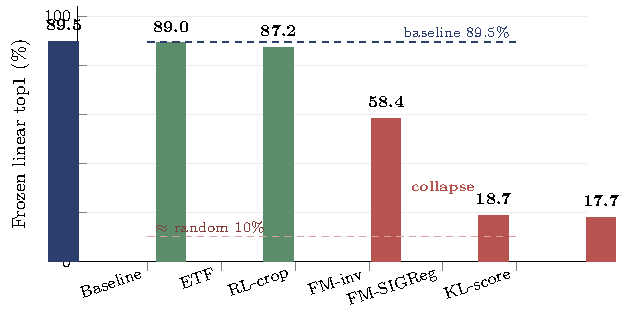
\includegraphics[width=\linewidth]{fig_climb_batch7_bars.pdf}

\vspace{0.2em}
{\scriptsize\color{mgray} Frozen linear top1 (best ckpt/idea); đường nét đứt = baseline 89.5\%.}

\column{0.42\textwidth}
\footnotesize
\textbf{\color{mprimary}Đọc kết quả:}\\[0.4em]
\scriptsize
\renewcommand{\arraystretch}{1.3}
\begin{tabular}{@{}l r l@{}}
\toprule
\textbf{Can thiệp} & \textbf{$\Delta$pp} & \textbf{Nhóm} \\
\midrule
\rowcolor{mgood!20} ETF head  & $-0.5$ & không đụng obj. \\
\rowcolor{mgood!11} RL-crop   & $-2.3$ & không đụng obj. \\
\rowcolor{mbad!12}  FM-inv    & $-31$  & thay invariance \\
\rowcolor{mbad!22}  FM-SIGReg & $-71$  & thay SIGReg \\
\rowcolor{mbad!32}  KL-score  & $-72$  & thay SIGReg \\
\bottomrule
\end{tabular}\\[0.55em]
{\scriptsize\color{mgray} klscore \& FM-SIGReg \emph{qua} được Phase-0 free-z gate nhưng full-train vẫn collapse.}

\end{columns}

\takeaway{Thay lõi SIGReg/invariance đều collapse — free-z hội tụ không kéo theo full-pipeline; đối chứng không đụng objective (ETF, RL-crop) giữ được baseline nhưng cũng không vượt. EppsPulley vẫn là neo.}

\end{frame}


% ─── CLIMB 5: Conv-stem architecture co-design ───────────────────────────────
\begin{frame}{Conv-stem: architecture co-design riêng}

\vfill
% Can thiệp: swap patchify → conv-stem
\begin{center}
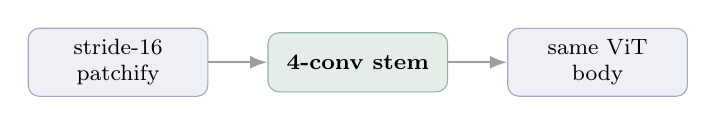
\begin{tikzpicture}[every node/.style={font=\footnotesize},
   b/.style={draw=mprimary!45, fill=mlight, rounded corners=4pt, minimum height=0.75cm,
             text width=2.0cm, align=center, inner sep=4pt},
   hl/.style={draw=mgood!65, fill=mlightsage, rounded corners=4pt, minimum height=0.75cm,
              text width=2.0cm, align=center, inner sep=4pt, font=\footnotesize\bfseries},
   ar/.style={-{Latex[length=2.2mm]}, thick, mgray}]
  \node[b] (p) {stride-16 patchify};
  \node[hl, right=0.75cm of p] (s) {4-conv stem};
  \node[b, right=0.75cm of s] (v) {same ViT body};
  \draw[ar] (p) -- (s);
  \draw[ar] (s) -- (v);
\end{tikzpicture}
\end{center}

\vspace{0.6em}
% Hero number
\begin{center}
{\fontsize{46}{50}\selectfont\bfseries\color{mgood!58!black}$\uparrow$\,+2.59\,pp}\\[10pt]
{\large\color{mprimary} Patchify \textbf{89.49\%}\;\; $\longrightarrow$\;\; Conv-stem \textbf{\color{mgood!58!black}92.08\%}}
\end{center}

\vspace{0.7em}
% Caveat chip
\begin{center}
\begin{tikzpicture}
  \node[draw=mbad!55, fill=mlightred, rounded corners=7pt, inner sep=7pt,
        text width=0.80\linewidth, align=center, font=\footnotesize]
   {\textbf{\color{mbad!75!black}Lưu ý:} cải thiện đến từ \emph{backbone inductive bias} — chưa phải bằng chứng objective LeJEPA tốt hơn.};
\end{tikzpicture}
\end{center}

\vspace{0.4em}
{\centering\scriptsize\color{mgray} Nguồn: Xiao et al., \emph{Early Convolutions Help Transformers See Better}, NeurIPS 2021 \citep{xiao2021early}. Thay patchify stride-16 bằng stem 4 conv; ViT body \& CLS giữ tương thích.\par}
\vfill

\takeaway{Headroom thật sự nằm ở kiến trúc đầu vào — không phải ở objective hay optimizer.}

\end{frame}


% ─── CLIMB 6: Synthesis ──────────────────────────────────────────────────────
\iffalse % ─── [HIDDEN] frame "Tổng hợp" ─────────────────────────────────────────
\begin{frame}{Tổng hợp: LeJEPA objective đã rất khó cải thiện trên fixed ViT-S}

\begin{columns}[T]
\column{0.50\textwidth}
\begin{primarybox}
\scriptsize
\textbf{Kết luận trên fixed ViT-S}\\[0.2em]
\begin{itemize}\itemsep3pt
  \item \textbf{Objective/head add-ons} không tạo winner rõ trước baseline 89.54\%.
  \item \textbf{Optimizer/training-geometry} không vượt được baseline 89.49\% một cách thuyết phục.
  \item Các thất bại vẫn có ý nghĩa: projector nhạy, auxiliary geometry có thể xung đột với SIGReg.
\end{itemize}
\end{primarybox}

\vspace{0.45em}
\begin{insightbox}
\scriptsize
\textbf{Headroom còn thấy được}\\[0.2em]
\kw{Architecture co-design}: conv-stem đạt \textbf{92.08\%} (\textbf{+2.59pp}) nhờ inductive bias đầu vào, cần track đánh giá riêng.
\end{insightbox}

\column{0.48\textwidth}
\begin{accentbox}
\scriptsize
\textbf{Thiếu bằng chứng trước khi claim rộng hơn}\\[0.2em]
\begin{itemize}\itemsep3pt
  \item multi-seed để tách nhiễu khỏi hiệu ứng thật;
  \item params/FLOPs cho conv-stem;
  \item same-stem baselines cho method không phải LeJEPA;
  \item frozen eval cho best pretrain checkpoint nếu bàn về early stopping/overfit.
\end{itemize}
\end{accentbox}

\vspace{0.45em}
\begin{badbox}
\scriptsize
\textbf{Không nên claim:} Conv-stem là cải thiện objective, hoặc các delta nhỏ là winner phổ quát ngoài setup Imagenette/frozen ViT-S này.
\end{badbox}

\end{columns}

\takeaway{Bức tranh hiện tại: objective LeJEPA đã khó cải thiện trên fixed ViT-S; headroom đáng theo đuổi nằm ở co-design kiến trúc và kiểm chứng mạnh hơn}

\end{frame}
\fi % ─── [HIDDEN] hết frame "Tổng hợp" ─────────────────────────────────────

% ═══ HẾT phần Nghiên cứu mở rộng ═══


% ─── Conclusion ───────────────────────────────────────────────────────────────
\begin{frame}[plain]
\begin{tikzpicture}[remember picture, overlay]
  % Nền tối full-bleed
  \fill[mdark] (current page.south west) rectangle (current page.north east);

  % Wordmark lệch trái-trên
  \node[anchor=north west, align=left, inner sep=0]
    at ([xshift=1.5cm, yshift=-1.9cm]current page.north west) {%
    {\bfseries\fontsize{42}{50}\selectfont\color{white}LeJEPA}\\[11pt]
    \textcolor{maccent}{\rule{2.8cm}{1.5pt}}\\[11pt]
    {\large\color{white!68}\addfontfeatures{LetterSpace=2.5}Từ heuristic đến lý thuyết}%
  };

  % Quote neo góc dưới-trái
  \node[anchor=south west, align=left, inner sep=0, text width=9.5cm]
    at ([xshift=1.5cm, yshift=1.9cm]current page.south west) {%
    {\itshape\large\color{white!82}``If 2024 was the year of scaling laws,\\[3pt]
    2025 may be the year we rediscover structure.''}%
  };

  % Q & A góc dưới-phải
  \node[anchor=south east, inner sep=0]
    at ([xshift=-1.6cm, yshift=1.9cm]current page.south east) {%
    {\LARGE\bfseries\color{maccent}\addfontfeatures{LetterSpace=5.0}Q \& A}%
  };
\end{tikzpicture}
\end{frame}
% ─── Glossary ─────────────────────────────────────────────────────────────────
\begin{frame}[allowframebreaks]{Phụ Lục: Bảng Tra Cứu Thuật Ngữ}
  \begin{primarybox}
  \footnotesize \textbf{Khái niệm Học máy \& Toán học cơ bản}
  \end{primarybox}
  \vspace{0.5em}
  {\scriptsize
  \renewcommand{\arraystretch}{1.4}
  \begin{tabular}{@{} >{\bfseries\color{mprimary}}l p{10.5cm} @{}}
    JEPA / LeJEPA & Joint-Embedding Predictive Architecture / Latent Epps-Pulley JEPA. \\
    SSL & Self-Supervised Learning (Học máy tự giám sát)\\
    Domain-specific SSL & Học tự giám sát đặc thù cho lĩnh vực cụ thể (huấn luyện trực tiếp trên dữ liệu chuyên biệt). \\
    Frontier transfer & Học chuyển giao từ các mô hình tiên tiến nhất (sử dụng mô hình nền tảng lớn đã huấn luyện sẵn). \\
    Downstream task & Tác vụ hạ nguồn (những tác vụ cụ thể áp dụng mô hình sau khi huấn luyện). \\
    Encoder / Predictor & Bộ mã hóa (trích xuất đặc trưng) / Bộ dự đoán. \\
    Embedding / Latent space & Vector nhúng / Không gian tiềm ẩn (nơi biểu diễn đặc trưng). \\
    Foundation model & Mô hình nền tảng (huấn luyện một lần, dùng cho nhiều tác vụ). \\
    Linear probe & Đánh giá mô hình bằng cách huấn luyện thêm một lớp tuyến tính đơn giản. \\
    Bias / Variance & Độ lệch (sai số hệ thống) / Phương sai (mức độ dao động của dự đoán). \\
    Anisotropic / Isotropic & Bất đẳng hướng (các hướng không đều) / Đẳng hướng (phân bố đều mọi hướng). \\
    Distribution / Gaussian & Phân phối / Phân phối chuẩn. \\
    Regularizer & Thành phần điều chuẩn (giúp định hình phân phối). \\
    Random projection & Phép chiếu ngẫu nhiên (chuyển không gian dữ liệu nhiều chiều xuống ít chiều hơn). \\
    Decision boundary & Ranh giới quyết định (đường/mặt phân tách các nhóm dữ liệu trong mô hình). \\
  \end{tabular}
  }

  \framebreak

  \begin{accentbox}
  \footnotesize \textbf{Đặc trưng \& Vấn đề trong LeJEPA}
  \end{accentbox}
  \vspace{0.5em}
  {\scriptsize
  \renewcommand{\arraystretch}{1.4}
  \begin{tabular}{@{} >{\bfseries\color{maccent!75!black}}l p{10.5cm} @{}}
    sync required & Yêu cầu đồng bộ dữ liệu. \\
    bottleneck — breaks DDP & Nút thắt cổ chai tính toán — phá vỡ quá trình huấn luyện song song. \\
    sub-gradient non-smooth & Sub-gradient không trơn (gây khó khăn cho việc tối ưu hóa). \\
    Bounded Gradient & Gradient (đạo hàm) bị chặn, ngăn chặn việc bùng nổ gradient. \\
    Curse of dimensionality & Lời nguyền số chiều (sự sụt giảm hiệu quả ở không gian nhiều chiều). \\
    Unified Error Bound & Chặn sai số thống nhất (cận trên của độ sai lệch phân phối). \\
    Scaling law & Quy luật mở rộng (mối quan hệ giữa quy mô mô hình/dữ liệu và hiệu năng). \\
    LeJEPA Generalizes VICReg & LeJEPA là một phiên bản tổng quát hóa của VICReg. \\
    Emergent semantics & Ngữ nghĩa nổi sinh (cấu trúc tự động phân tách mà không cần nhãn). \\
    Sweet spot & Điểm cân bằng lý tưởng (giá trị siêu tham số tối ưu). \\
    Fixed / Resampled (SGD) & Tập hướng chiếu cố định / Lấy mẫu lại liên tục qua từng bước SGD. \\
    Differentiable sort relaxation & Kỹ thuật xấp xỉ thao tác sắp xếp để có thể tính được vi phân. \\
  \end{tabular}
  }
\end{frame}

% ─── References ───────────────────────────────────────────────────────────────
\begin{frame}[allowframebreaks]{Tài Liệu Tham Khảo}
\nocite{*}
\bibliographystyle{plainnat}
\bibliography{references}
\end{frame}

\end{document}
